\cotefile{29}
\scanpage{49}
% archive foliation: 46 (pencil, lower left; uncertain)
\begin{center}- 23 -\end{center}
\begin{flushright}n°385\end{flushright}

\uline{l'injection de} $Y$ \uline{dans} $X$. \uline{Pour tout point} $a$ \uline{de} $Y$, \uline{l'application} $\iota_a$ \uline{est une bijection de} $D_a(Y)$ \uline{sur le sous-espace de} $D_a(X)$ \uline{constitué des} $\mu$ \uline{telles que} $f.\mu=0$ \uline{pour toute fonction de classe} $C^r$ \uline{dans un voisinage} $U$ \uline{de} $a$, \uline{nulle en tout point de} $Y\cap U$.

Soit $\mu$ dans $D_a(Y)$ et $f$ de classe $C^r$ dans un voisinage $U$ de $a$, nulle sur $Y\cap U$ ; on a :
\[
f.\iota_a(\mu)=\iota_a((f\circ\iota).\mu)=0
\]
puisque $f\circ\iota=0$. Comme $Y$ est une sous-variété de $X$, il existe un ouvert $U$ contenant $a$, un système de coordonnées $x_1,\ldots,x_n$ dans $U$, et un entier $m$ tel que $0\leq m\leq n$ et que $Y\cap U$ soit l'ensemble des points de $U$ où s'annulent $x_{m+1},x_{m+2},\ldots,x_n$. Les fonctions $x_1\circ\iota,\ldots,x_m\circ\iota$ forment alors un système de coordonnées sur l'ouvert $Y\cap U$ de $Y$.

L'espace $D_a(Y)$ a une base $\{\Lambda^\alpha\}_{\alpha\in\unsure{\mathbf{N}|\mathbb{N}}_r^m}$ caractérisée par :
\[
\langle\Lambda^\alpha,x^{\alpha'}\circ\iota\rangle=\delta_{\alpha\alpha'}
\qquad \alpha,\alpha'\in\unsure{\mathbf{N}|\mathbb{N}}_r^m
\]
et l'espace $D_a(X)$ admet une base $\{\Delta^\beta\}_{\beta\in\unsure{\mathbf{N}|\mathbb{N}}_r^n}$ définie par :
\[
\langle\Delta^\beta,x^{\beta'}\rangle=\delta_{\beta\beta'}
\qquad \beta,\beta'\in\unsure{\mathbf{N}|\mathbb{N}}_r^n.
\]
Nous noterons $0$ l'élément nul de $\unsure{\mathbf{N}|\mathbb{N}}_r^{n-m}$ ; on a alors $\iota_a(\Lambda^\alpha)=\Delta^{(\alpha,0)}$ pour tout $\alpha$ dans $\unsure{\mathbf{N}|\mathbb{N}}_r^m$ et par conséquent, $\iota_a$ est injective.

Par ailleurs, soit $\mu$ dans $D_a(X)$ telle que $x_i.\mu=0$ pour $m<i\leq n$. D'après (59), on en déduit $\langle\mu,x^\beta\rangle=0$ pour tout multiindice $\beta$ dans $\unsure{\mathbf{N}|\mathbb{N}}_r^n$ pour lequel il existe $i$ avec $m<i\leq n$ et $\beta_i\neq0$ ; autrement dit, on ne peut avoir $\langle\mu,x^\beta\rangle\neq0$ que si $\beta=(\alpha,0)$ pour $\alpha$ dans $\unsure{\mathbf{N}|\mathbb{N}}_r^m$ convenable. De la formule $\mu=\sum_\beta\langle\mu,x^\beta\rangle.\Delta^\beta$, on déduit alors $\mu=\sum_\alpha\langle\mu,x^\alpha\rangle\,\iota_a(\Lambda^\alpha)$, ce qui prouve que $\mu$ est dans l'image de $\iota_a$.
\begin{flushright}C.Q.F.D.\end{flushright}

Pour tout point $a$ de $X$, l'espace vectoriel $D_a(X)\otimes D_a(X)$ est muni d'une structure

\scanpage{50}
\mspage{II}
% archive foliation: 49
Soit $Y_1$ le \unsure{normalisé|localisé} de $Y$ en $y$,
\inserted{\unsure{pour des points étales}}
\deleted{\unsure{Alors}}
\inserted{en \unsure{le} $y\in Y$.}
\inserted{\unsure{Quant à} \deleted{\unsure{localisation}} \unsure{en un} \deleted{\unsure{V}} \unsure{voisinage de la fibre} \deleted{\unsure{spéciale}}}
\deleted{$X$ \unsure{étant} \inserted{\unsure{en} $X_y$} \unsure{le même sur} $Y$ \unsure{alors} $X_1=X\times_Y Y_1$ \unsure{le est sur}}
\inserted{\unsure{on peut supposer} $X_y$ \deleted{\unsure{fibre spéciale}} \unsure{connexe}. Donc, il \unsure{nous est}}
\deleted{$Y_1$, $X_1$ \illegible{2}, \unsure{donc} \illegible{3}}
\inserted{\unsure{au cas de} $X_1=X\times_Y Y_1$, \unsure{notre} $y$ \unsure{induit un morphisme dans}}
\unsure{alors de} $X_1$, \unsure{et}
\inserted{\unsure{le même}}
\unsure{considérons sur la fibre} géométrique \unsure{en} $Z_y$, il s'\unsure{ensuit}
\inserted{un $X$-\unsure{morphisme} $X_1\leftarrow Z$ \unsure{qui}}
\unsure{fait un isom sur la fibre de} $(X_1)_y$.

\diagram{\begin{tikzcd}[row sep=large,column sep=large]
X \arrow[dd] & \\
& X_1 \arrow[ul] \arrow[dd] \\
Y & \\
& Y_1 \arrow[ul]
\end{tikzcd}}

\deleted{(\unsure{car par} \illegible{1} $Z$ \unsure{de} \illegible{1}, $X_1$ \unsure{est étale}}
\inserted{j'\unsure{ajoute que} $X_1$ \unsure{est étale sur} $Y$ \unsure{sur la fibre}}
\deleted{\unsure{sur} $X$, $Y_1\to$\unsure{étale} \unsure{sur} $Y$.}
\inserted{\unsure{en} $Y_1$, \unsure{comme pointé}.}
Donc \unsure{on a}
\[
Z\simeq X\times_Y Y_1,\quad Y_1\ \text{\unsure{revêtement} fini étale de }Y.
\]

Par \unsure{suite} (\unsure{comme on a prouvé}), \deleted{\unsure{$X_1$ est}}
$X_1$ est étale sur $X$, \unsure{partout}, et \deleted{\unsure{les morphismes}}
\inserted{des \unsure{considérations}}
de \unsure{profondeur} nous donnent un $X$-isom
\[
X_1\simeq Z,
\]
ce qui achève la démonstration.

\uline{NB} \unsure{Ceci prouve} plus qu'on n'avait annoncé, savoir ceci : une suite exacte de
\margin{\deleted{\unsure{R}}}
\margin{\figure{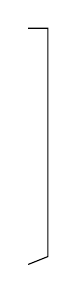
\begin{tikzpicture}
\draw (0,0)--(.25,0)--(.25,-2.9)--(0,-3);
\end{tikzpicture}}}
\diagram{\begin{tikzcd}[column sep=large]
\pi_1(X_{\bar y},\unsure{\xi}) \arrow[r,dash] &
\pi_1(X,\unsure{\xi}) \arrow[r] &
\pi_1(Y,\unsure{\eta}) \arrow[r] & 0
\end{tikzcd}}

\deleted{\unsure{Cela}}
généralise (\unsure{en dehors} l'hyp. noethérienne)
SGA IX 6.1, 6.2. \ldots\ Ne pas confondre avec les résultats de SGA X, où on prend une fibre \unsure{pas}%
\inserted{\uline{\unsure{néc|ici}}}%
\uline{générique} (en revanche, il y faut \unsure{je crois} que $f$ \unsure{soit} propre \ldots).

\scanpage{51}
\begin{center}- 22 -\end{center}
\begin{flushright}n°385\end{flushright}
\[
\begin{aligned}
\langle\varphi_*(\mu),fg\rangle
&=\langle\mu,(f\circ\varphi)(g\circ\varphi)\rangle
=\sum\langle\mu'_i,f\circ\varphi\rangle\langle\mu''_i,g\circ\varphi\rangle\\
&=\sum\langle\varphi_*\mu'_i,f\rangle\langle\varphi_*\mu''_i,g\rangle
\end{aligned}
\]
et par suite :
\[
P\varphi_*(\mu)=\sum\varphi_*\mu'_i\otimes\varphi_*\mu''_i
=(\varphi_*\otimes\varphi_*)(P(\mu)).
\]

10. \uline{Produit d'une fonction et d'une distribution}.

Soit $a$ un point de $X$. Le dual $V$ de l'algèbre commutative $C_a^r(X)$ est muni d'une structure de module sur $C_a^r(X)$ définie par la formule :
\[
(59)\qquad \langle f.\mu,g\rangle=\langle\mu,fg\rangle
\qquad \mu\in V,\ f,g\in C_a^r(X).
\]
Comme $D_a^k(X)$ est le sous-espace de $V$ formé des formes linéaires nulles sur l'\uline{idéal} $I_a^{k+1}(X)$, c'est un sous-module de $V$. Comme $D_a(X)$ est la réunion des espaces $D_a^k(X)$ pour les entiers $k\leq r$, on voit que la formule (59) définit sur $D_a(X)$ une structure de module sur l'anneau $C_a^r(X)$.

Pour tout ouvert $U$ de $X$, on définit comme suit une structure de $C^r(U)$-module sur l'ensemble des distributions de support contenu dans $U$ ; pour $f$ dans $C^r(U)$ et une distribution $\mu$ avec $S(\mu)\subset U$, on pose :
\[
(f.\mu)_a=
\begin{cases}
\gamma_a(f).\mu_a&\text{si }a\in U\\[1ex]
0&\text{si }a\notin U.
\end{cases}
\]
La formule (59) reste valable pour $f,g$ dans $C^r(U)$ si $S(\mu)\subset U$.

Etant données une variété $Y$ de classe $C^r$, un morphisme $\varphi$ de $Y$ dans $X$, $\mu$ dans $D(X)$, $\unsure{\nu}$ dans $D(Y)$, $f$ dans $C^r(X)$ et $g$ dans $C^r(Y)$, on a les relations :
\[
(60)\qquad (f.\mu)\times(g.\unsure{\nu})=(f\times g).(\mu\times\unsure{\nu})
\]
\[
(61)\qquad \varphi_*((f\circ\varphi).\unsure{\nu})=f.\varphi_*(\unsure{\nu}).
\]

PROPOSITION 6.-- \uline{Soient} $X$ \uline{une variété de classe} $C^r$, $Y$ \uline{une sous-variété de} $X$, \uline{et} $\iota$

\scanpage{52}
\mspage{\unsure{III|II}}
% archive foliation: 51
\uline{Lemme 2} Soit $X\to Y$ un morphisme de type fini, avec $Y$ loc. noeth. et univ. japonais.
Alors pour tt faisceau d'ensembles constructible $F$ sur $X$, $f_*(F)$ est constructible.

\unsure{SGA|§ A} au début

\uline{Lemme 3} $X$ schéma connexe \deleted{\unsure{loc}} noeth.,
\inserted{univ. japonais},
$(X_i)_{i\in I}$ une partition finie en parties loc. fermées, $G$ un groupe fini.
\deleted{Supposons que pour tout $i$, $H^1(X_i,G)$ soit fini.}
\inserted{Considérons l'\deleted{\unsure{application}}}
\deleted{Alors \unsure{pour tt}}
\diagram{\begin{tikzcd}
H^1(X,G)\arrow[r]&\displaystyle\prod_i H^1(X_i,G)
\end{tikzcd}}
Cette application est à \uline{fibres finies}. En particulier, si pour tt $i$, $H^1(X_i,G)$ est fini, kif kif pour $H^1(X,G)$.

\unsure{Théorie du recollement} des faisceaux étales, en utilisant lemme 2 et le fait suivant :
\inserted{\uline{Lemme 4}}
Si $F,G$ sont des faisceaux \inserted{d'ens} étales constr. sur $X$ noethérien, alors $\operatorname{Hom}(F,G)$ est un ens fini.
\margin{\figure{\begin{tikzpicture}
\draw (0,0)--(0,-1.2);
\end{tikzpicture}}}

\deleted{\unsure{Corollaire}}
\deleted{\unsure{Proposition}}
\inserted{\uline{Proposition}}
$S$ \deleted{\unsure{X}} schéma noeth. univ. japonais,
$G$ un groupe fini. Conditions équivalentes.

\scanpage{53}
% archive foliation: 52
\begin{center}- 13 -\end{center}
\begin{flushright}n°385\end{flushright}
7. \uline{Produit cartésien de deux distributions}.

Soient $X$ et $Y$ deux variétés de classe $C^r$, $a$ un point de $X$ et $b$ un point de $Y$.
Il existe une application linéaire $\iota$ de $D_a^r(X)\otimes D_b^r(Y)$ dans l'espace $B$ des formes bilinéaires sur $C_a^r(X)\times C_b^r(Y)$ caractérisée par la formule :
\[
(31)\qquad \iota(\mu\otimes\unsure{\nu})(f,g)=\langle\mu,f\rangle\langle\unsure{\nu},g\rangle.
\]
Par ailleurs, on définit une application linéaire $\iota'$ de $D_{a,b}^r(X\times Y)$ dans $B$ par la formule :
\[
(32)\qquad \iota'(\pi)(f,g)=\langle\pi,f\times g\rangle.
\]

PROPOSITION 4.-- \uline{Il existe une application linéaire} $\rho_{a,b}$ \uline{de} $D_{a,b}^r(X\times Y)$ \uline{dans} $D_a^r(X)\otimes D_b^r(Y)$ \uline{et une seule telle que} $\iota'=\iota\circ\rho_{a,b}$. \uline{L'application} $\rho_{a,b}$ \uline{est injective et son image est le sous-espace de} $D_a^r(X)\otimes D_b^r(Y)$ \uline{engendré par les éléments} $\mu\otimes\unsure{\nu}$ \uline{avec} $v(\mu)+v(\unsure{\nu})\leq r$. \uline{En particulier, si} $r$ \uline{n'est pas un entier, l'application} $\rho_{a,b}$ \uline{est bijective}.

Nous introduirons un système de coordonnées $x_1,\ldots,x_n$ sur $X$ au voisinage de $a$ et tel que $x_i(a)=0$ pour tout $i$ ; de même, on introduit un système de coordonnées $y_1,\ldots,y_m$ sur $Y$ au voisinage de $b$ tel que $y_j(b)=0$ pour tout $j$. D'après la prop.2 il existe des bases $\{\Delta_a^\alpha\}$ de $D_a^r(X)$ et $\{\Delta_b^\beta\}$ de $D_b^r(Y)$ caractérisées par les formules :
\[
(33)\qquad
\langle\Delta_a^\alpha,x^{\alpha'}\rangle=\delta_{\alpha\alpha'}
\qquad
\langle\Delta_b^\beta,y^{\beta'}\rangle=\delta_{\beta\beta'}
\]
pour $\alpha$ et $\alpha'$ dans $\unsure{\mathbf{N}|\mathbb{N}}_r^n$ et $\beta$ et $\beta'$ dans $\unsure{\mathbf{N}|\mathbb{N}}_r^m$. Par conséquent, le produit tensoriel $D_a^r(X)\otimes D_b^r(Y)$ admet pour base les éléments $\Delta_a^\alpha\otimes\Delta_b^\beta$ pour $\alpha$ dans $\unsure{\mathbf{N}|\mathbb{N}}_r^n$ et $\beta$ dans $\unsure{\mathbf{N}|\mathbb{N}}_r^m$.

Par ailleurs (référence), on définit un système de coordonnées $z_1,\ldots,z_{n+m}$ sur $X\times Y$ au voisinage de $(a,b)$ par les conditions :

\scanpage{54}
\mspage{IV}
% archive foliation: 53
(i) Pour tout $X$ de t.f. sur $S$, $H^1(X,G)$ est fini.

(ii) Pour tt sous-schéma \deleted{\unsure{affine}} normal
\inserted{\unsure{intègre affine}}
\deleted{\unsure{de }$S$}
$S_0$ de $S$, \deleted{\unsure{et}} tt \unsure{rev.} fini étale
$S'$ de $S_0$, tout schéma \inserted{affine} lisse de t. fini $X$ sur $S'$, à fibres géom. connexes non vides, $H^1(\unsure{X},G)$ est fini.

(iii) Pour tt $S',X$ comme dessus, $S'\neq\varnothing$, il existe un ouvert non vide $U$ de $S'$ tel que $H^1(X|\unsure{U'|U},G)$ \unsure{soit} fini.

Il \uuline{suffit} pour ceci qu'on ait ceci :

(iv) a) Pour tout $s\in S$, et tt schéma $\bar X$ de type fini lisse affine connexe sur $\overline{k(s)}$,
\[
H^1(\bar X,G)\text{ est fini}
\]

b) Pour tout \deleted{\unsure{$S$}} \deleted{\unsure{un}} schéma affine normal intègre $S'$ \deleted{de $S$},
\inserted{comme dans (ii)}
et tt sous groupe $H$ de $G\times G$,
\deleted{\illegible{1}}
$H^1(S',H)$ est fini.

Lorsque $G$ est commutatif, on peut affaiblir b) en y remplaçant $H$ par $G$.

\figure{\begin{tikzpicture}
\draw (0,0)--(3.2,0);
\end{tikzpicture}}

\uline{Dém.} Equivalence de (i) à (iii) résulte aussitôt de lemme 3. Pour prouver qu'\unsure{ils} sont entrainés par (iv), on doit utiliser en plus lemme 1.

\scanpage{55}
% archive foliation: 54
\begin{center}- 12 -\end{center}
\begin{flushright}n°385\end{flushright}
\uline{caractérisé par la propriété suivante} :

\uline{Pour tout} $\mu$ \uline{dans} $\bar D_a^1(X)$ \uline{et tout système de coordonnées} $x_1,\ldots,x_n$ \uline{au voisinage de} $a$, \uline{le vecteur tangent} $u(\mu)$ \uline{admet les composantes} $\langle\mu,x_1\rangle,\ldots,\langle\mu,x_n\rangle$ \uline{par rapport au système de coordonnées} $x_1,\ldots,x_n$.

Nous allons, pour terminer ce n°, examiner l'effet d'un morphisme sur une distribution d'ordre 1.

Soit $\varphi$ un morphisme de $X$ dans une variété $X'$ de classe $C^r$. Soit $x_1,\ldots,x_n$ un système de coordonnées au voisinage d'un point $a$ de $X$, et $x'_1,\ldots,x'_m$ un système de coordonnées sur $X'$ au voisinage du point $a'=\varphi(a)$. Le morphisme $\varphi$ s'exprime dans ces systèmes de coordonnées par les formules :
\[
(28)\qquad x'_j(\varphi(p))=\varphi_j(x_1(p),\ldots,x_n(p))
\qquad 1\leq j\leq m.
\]
D'après les formules (15) et (24), on a alors :
\[
(29)\qquad
\langle\varphi_a\mu,x'_j\rangle
=\sum_{1\leq i\leq n}\langle\mu,x_i\rangle\,D_i\varphi_j(x_1(a),\ldots,x_n(a))
\qquad 1\leq j\leq m
\]
pour toute distribution $\mu\in L$ ; le premier membre de cette formule représente la j-ième composante du vecteur tangent $u_{\varphi(a)}(\varphi_a(\mu))$ dans le système de coordonnées $x'_1,\ldots,x'_m$, et, par définition de l'application $T_a(\varphi)$, le second membre de (29) représente la j-ième composante du vecteur tangent $(T_a(\varphi)\circ u_a)(\mu)$ dans le même système de coordonnées sur $X'$. Autrement dit, on a :
\[
(30)\qquad u_{\varphi(a)}\circ\varphi_a=T_a(\varphi)\circ u_a.
\]

Nous identifierons désormais les espaces $\bar D_a^1(X)$ et $T_a(X)$ au moyen de l'isomorphisme $u_a$ précédent, lorsque $r\neq\unsure{\omega|0}$.

\uline{Remarque}.-- Lorsque $r=\unsure{\omega|0}$, l'espace $T_a(X)$ n'a pas été défini précédemment [et pour cause !] ; nous poserons par définition $T_a(X)=\bar D_a^1(X)$, et $T_a(\varphi)=\varphi_a$. La formule (27) reste valable si l'on définit la matrice jacobienne par $J_{i,j}(a)=(D_i)_a y_j$, la base $(D_i)_a$ de $\bar D_a^1(X)$ étant définie par $\langle(D_i)_a,x_j\rangle=\delta_{i,j}$.

\scanpage{56}
\mspage{V}
% archive foliation: 55
\uline{Cor} 1 Supposons que $G$ soit premier aux car. résiduelles.
\deleted{Alors \unsure{on}}
Supposons que pour tt sous-schéma affine intègre normal $S_0$ de $S$, et tt \uline{revêt} \uline{étale} $S'$ \inserted{intègre} de $S_0$, enfin tt sous-groupe $H$ de $G\times G$, on ait $H^1(S',H)$ fini.
Alors pour tt $X$ de t.f. sur $S$, $H^1(X,G)$ est fini.

Si $G$ est commutatif, il suffit de faire $H=G$ (\unsure{c'est} une condition \unsure{néce|nécessaire} et suffisante).

\uline{Corollaire} 2 Conditions équivalentes.

(i) Pour tt $X$ de t.f. sur $Y$, et tt groupe \inserted{fini} $G$ premier aux car. résiduelles de $X$, on a $H^1(X,G)$ fini.

(ii) \deleted{\unsure{Pour}} Idem avec $X$ revêt \deleted{fini} étale intègre d'un sous-schéma affine normal intègre $S_0$ de $S$.

\uline{NB} Dans le cor. 1, on a utilisé le fait que si $k$ est un corps alg. clos, alors pour tt $X$ de t.f. sur $k$ et $G$ premier à la car. de $k$, $H^1(X,G)$ est fini.
Voyons comment cela peut être prouvé par les méthodes envisagées ici.

\scanpage{57}
% archive foliation: 56
\begin{center}- 11 -\end{center}
\begin{flushright}n°385\end{flushright}
$\Psi_i$ et $\Psi'_i$ définies et continues dans un voisinage du point $\xi=(x_1(a),\ldots,x_n(a))$ de $K^n$ et telles que :
\[
\Phi=\sum_i\Psi_i\Psi'_i
\qquad \Psi_i(\xi)=\Psi'_i(\xi)=0
\]
et que les $\Psi_i$ soient de classe $C^r$. Ces conditions entraînent que
$\Phi(\lambda_1,\ldots,\lambda_n)/\sum_i|\lambda_i-\xi_i|$ tend vers $0$ si le point $(\lambda_1,\ldots,\lambda_n)$ tend vers $\xi$, et par conséquent que les dérivées de $\Phi$ sont nulles au point $\xi$. Comme on a par ailleurs $\langle\mu,f\rangle=0$ dans ce cas, la formule (24) est encore vraie.

La prop.1 montre que tout élément de $C_a^r(X)$ est congru modulo $I_a^2(X)$ au germe en $a$ d'un polynôme de degré $\leq1$ en les $x_i$ ; les cas particuliers précédemment démontrés prouvent que (24) est vraie en général.
\begin{flushright}C.Q.F.D.\end{flushright}

Considérons alors deux systèmes de coordonnées $x_1,\ldots,x_n$ et $y_1,\ldots,y_n$ au voisinage du point $a$ ; nous introduirons les fonctions de passage $\Phi_j$ telles que l'on ait :
\[
(26)\qquad y_j(p)=\Phi_j(x_1(p),\ldots,x_n(p))
\qquad 1\leq j\leq n
\]
lorsque $p$ appartient à l'intersection des domaines de définition des deux systèmes de coordonnées ; par ailleurs, on introduit la matrice jacobienne par :
\[
J_{ij}(p)=D_i\Phi_j(x_1(p),\ldots,x_n(p)).
\]
D'après le lemme 1 appliqué à $f=y_j$, on a alors :
\[
(27)\qquad
\langle\mu,y_j\rangle=\sum_{1\leq i\leq n}\langle\mu,x_i\rangle J_{ij}(a)
\qquad 1\leq j\leq n
\]
pour tout $\mu\in L$. D'après la définition d'un vecteur tangent, on a finalement la proposition suivante :

PROPOSITION 3.-- \uline{Soient} $a$ \uline{un point d'une variété} $X$ \uline{de classe} $C^r$ $(r\neq\unsure{\omega|0})$, \uline{et} $\bar D_a^1(X)$ \uline{l'espace des distributions} $\mu$ \uline{de support} $a$ \uline{et d'ordre} $\leq1$ \uline{telles que} $\langle\mu,1\rangle=0$.
\uline{Il existe un isomorphisme} $u$ \uline{de} $\bar D_a^1(X)$ \uline{sur l'espace tangent} $T_a(X)$ \uline{à} $X$ \uline{au point} $a$,

\scanpage{58}
\mspage{VI}
% archive foliation: 57
\deleted{\unsure{On est}}
Récurrence sur $\dim X$.
\inserted{trivial si $\dim\leq0$.}
\deleted{\unsure{Utilisant}}
\deleted{\unsure{on a}}
lemme 3, on est ramené au cas où $X$ est lisse et
\inserted{connexe. Si $\dim X=1$,}
\deleted{\unsure{admet un morphisme lisse surjectif}}
c'est facile (réduction au cas compact par lemme de Abhyankar)
\deleted{\unsure{et}}
c'est dû à Serre-Lang.
\deleted{\unsure{D'une manière}}

Si $\dim X\geq2$, on est ramené \deleted{\unsure{au cas}}
\inserted{\unsure{par}}
lemme 3, au cas où il y a une fibration \inserted{lisse} $X\to Y$, $\dim Y<\dim X$, \deleted{\unsure{et}}
\unsure{qui est} à fibres géom. connexes non vides, de dim 1.
On applique alors le lemme 1 et la hyp. de récurrence.

\margin{?}
\uline{Prop} Soit $k$ un corps. On suppose que pour tt \deleted{\unsure{$X$}}
courbe \inserted{\unsure{alg.}} lisse $X$ sur $k$, le nb de rev. étales de $X$ de degré donné est fini.
Alors la $=$ chose est \unsure{vrai|vraie} pour \uline{tt} $X$ de t.f. sur $k$.

\scanpage{59}
% archive foliation: 58
\begin{center}-10-\end{center}
\begin{flushright}n°385\end{flushright}
dans un voisinage ouvert de $a$. En particulier on a $\varepsilon_a=\Delta_a^0$.

6. \uline{Distributions et vecteurs tangents}.

La proposition 2 montre comment un système de coordonnées au voisinage d'un point $a$ de $X$ définit une base de l'espace des distributions de support $a$ ; cette base dépend du système de coordonnées choisi. Nous allons étudier comment varient les éléments d'ordre 1 de la base en fonction du système de coordonnées. \uline{Nous supposerons} $r\neq\unsure{\omega|0}$.

Soient $a$ un point de $X$ et $L$ l'espace vectoriel $\bar D_a^1(X)$. Comme on a $\langle\mu,f\rangle=0$ pour toute distribution $\mu\in L$ et toute fonction constante $f$, la prop.2 montre que l'application :
\[
(22)\qquad \mu\longrightarrow(\langle\mu,x_1\rangle,\ldots,\langle\mu,x_n\rangle)
\]
est un isomorphisme de $L$ sur $K^n$ quel que soit le système de coordonnées $x_1,\ldots,x_n$ sur $X$ au voisinage de $a$. On peut par contre définir une base $(D_i)_a$ de $\bar D_a^1(X)$ par $\langle(D_i)_a,x_j\rangle=\delta_{i,j}$. On a donc $(D_i)_a=\Delta_a^\alpha$ avec $\alpha=e_i$. On a de plus le résultat suivant :

LEMME 1.-- \uline{Soit} $f$ \uline{une fonction de classe} $C^r$ \uline{définie dans un voisinage ouvert} $V$ \uline{de} $a$ \uline{contenu dans} $U$, \uline{et soit} $\mu$ \uline{dans} $L$. \uline{Si} $f$ \uline{est de la forme} :
\[
(23)\qquad f(p)=\Phi(x_1(p),\ldots,x_n(p))
\qquad p\in V
\]
\uline{et si} $D_i\Phi$ \uline{est la dérivée de la fonction} $\Phi$ \uline{par rapport à la i-ème variable, on a} :
\[
(24)\qquad
\langle\mu,f\rangle=\sum_{1\leq i\leq n}\langle\mu,x_i\rangle\,D_i\Phi(x_1(a),\ldots,x_n(a))
\]
\uline{et en particulier}
\[
(25)\qquad
\langle(D_i)_a,f\rangle=D_i\Phi(x_1(a),\ldots,x_n(a))
\qquad 1\leq i\leq n.
\]

La formule (24) est évidemment satisfaite si $f=1$, ou si $f=x_i$. Supposons maintenant que le germe de $f$ en $a$ soit dans $I_a^2(X)$ ; il existe alors des fonctions

\scanpage{60}
% archive foliation: 59
\begin{flushright}
$\pi_1$ et \uline{Pic}$^\tau$ birationnels
\end{flushright}

\scanpage{61}
\mspage{1.}
% archive foliation: 60
\uline{Th.} Soit $X$ préschéma alg., sur $k$ alg. clos. Alors
\[
\pi'_1(X)=\text{limite projective des groupes quotients discrets de }\pi_1(X)
\text{ d'ordres premiers à }p
\]
est top. de type fini.

Grace à ``van Kampen'', on peut supposer $X$ affine
\inserted{\deleted{\unsure{intègre}}\unsure{et réduit}},
puis $X$ affine et \uline{normal}
[sinon, on aura
\diagram{\begin{tikzcd}
X'\times_X X' \arrow[r,shift left=.5ex] \arrow[r,shift right=.5ex] & X' \arrow[r] & X
\end{tikzcd}}
, et $\pi_1(X)$ est engendré par $\pi_1(X')$ et un nb fini de générateurs
correspondants aux composantes irrédu. de $X'\times_X X'$, donc il en est de $=$
de $\pi'_1(X)$
\inserted{\unsure{par $\pi'_1(X')$ et \ldots}}
(\unsure{car cela se prouve|car cela est} pour les grps profinis,
\unsure{voir $(\varphi)$}). 

Si $\dim X=0$, trivial

Si $\dim X=1$, théorie de la spécialisation du groupe fondamental
\margin{\figure{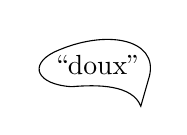
\begin{tikzpicture}[scale=.55]\draw (0,0) .. controls (-.8,.05) and (-1,.5) .. (-.4,.8) .. controls (.8,1.35) and (2,1.1) .. (1.8,.25) -- (1.6,-.45) .. controls (1.4,.05) and (.6,.05) .. (0,0);\node at (.6,.5) {``doux''};\end{tikzpicture}}}
nous ramène au cas de la \unsure{car.ctéristique|caractéristique} $0$, où on a
\deleted{\unsure{un}}\deleted{\unsure{le groupe}}
\inserted{le résultat} par voie transcendante.

Si $\dim X\geq2$, on considère une immersion
\[
X^n\longrightarrow \unsure{\mathbf P|P}_k^r
\]
et un \unsure{hyperplan} \deleted{\unsure{générique}}
\inserted{\unsure{variété lin gén} $L^{r-n+1}$}, défini sur une
ext. alg close $K$ de $k$, on pose
\[
C=\deleted{\unsure{\mathbf P_k^r|P_k^r}}X^n\times_{\unsure{\mathbf P|P}_k^r}L^{r-n+1}
\]
qui est une courbe normale de dim $1$ sur $K$, et alors en vertu de
Bertini ``générique'',
\diagram{\begin{tikzcd}\pi_1(C)\arrow[r]&\pi_1(X)\end{tikzcd}}
est \uline{surjectif}. [Réf]. Donc $\pi'_1(C)-\pi'_1(X)$ l'est
aussi, OK.

\uline{Question} $X$ normal complet, $Y\subset X$
\deleted{\unsure{de codim $\geq1$}}
Alors $\pi_1(X-Y)$ mod le sous-groupe invariant fermé engendré
par les groupes d'inertie wild en les composantes de
\deleted{\unsure{degré}}
codim $1$ de $Y$, est de top. de type fini ??

\scanpage{62}
\mspage{2.}
% archive foliation: 61
\uline{Question}
\deleted{\unsure{Soit} $X,\unsure{E}$ \unsure{un préschéma alg. sur}}
$k$ alg. clos,
\deleted{\unsure{type fini sur $k$}}
$X$ \deleted{complet}\inserted{\unsure{propre sur $k$}},
\deleted{\unsure{$X'$}}
$D$ une partie fermée de $X$, \deleted{$U=X-Y$}

$X'$ le normalisé de $X_{\mathrm{réd}}$,
$\unsure{D'_i|D_i}$ les composantes irréductibles de codim $1$ de
$p^{-1}(D)$,
\inserted{$d_i$ le pt gén. de $\unsure{D'_i|D_i}$},
$U=X-D$,
\margin{\diagram{\begin{tikzcd}
X'\arrow[d,"p"'] & \unsure{D'_i}\arrow[l,phantom,"\supset" description]\arrow[d]\\
X & D\arrow[l,phantom,"\supset" description]
\end{tikzcd}}}

$Y$ un préschém. \deleted{\unsure{alg.}}
\inserted{localement \unsure{noethérien}},
\inserted{$P=Y\times U$, $P'=Y\times U'$},
$Q$ un revêtement étale de
\deleted{$\unsure{Y}\times\unsure{U}$}\inserted{$P$},
\deleted{$\unsure{Y_k}$}
\inserted{$y\in Y(k)$}.
On suppose

(i) $Q\times_P P'$ est \inserted{\uuline{\unsure{géométr.}}}
\uline{tamely ramifié} en les
\inserted{$\unsure{D_i|d_i}\times_k k(\eta)$,
$\eta$ \deleted{\unsure{les points}} les pts gén. des comp. irrédu. de $Y$.}
\deleted{\unsure{fini.}}
\deleted{[NB Si $Y$ est \unsure{réduit}, il suffit \unsure{de}]}

(ii) $Q\times_Y y$ est un rev. \uline{trivial} de $U$.

\margin{\diagram{\begin{tikzcd}
P'=Y\times U'\arrow[d]\arrow[r,hook]&Y\times X'=Q'\arrow[d]\\
\deleted{\unsure{Y\times D'}}\,P=Y\times U\arrow[r,hook]\arrow[d]&Y\times X=Q\\
Y&
\end{tikzcd}}}

Alors \deleted{pour tt $y'\in Y$, $Q_{y'}$ est un \unsure{rev.}}
\inserted{Il existe un rev. étale $Q_0$ \deleted{\unsure{sur}}
\inserted{d'un voisinage \unsure{de $y$}} et}
un $P$-isom
\[
\deleted{\unsure{Q(P')}\,\unsure{Q_0\times_Y P'}}\quad
Q\simeq Q_0\times_Y P=Q_0\times U.
\]
\deleted{\unsure{Quid?}\quad\unsure{$U_{\bar k}$ géo.}}
\inserted{\unsure{$Q_0\times_Y k(y'),\ Q_{y'}$ est}}
\margin{\unsure{(On sait [inf])}}
\unsure{qui est VU de même pour tout $y'$}
\deleted{\unsure{fermé}},
\unsure{un rev. trivial de $k(y')$. On peut donc supposer $Y$ de sorte à ses composantes
irrédu. distinctes.}

Supposons d'abord $X$ normal, i.e. $X=X'$.
\deleted{Soit} La question étant
\inserted{\unsure{pure|donc}}``\unsure{birat.elle|biréelle}'' sur les fibres,
on peut supposer $X$ affine, alors \unsure{fixons} une immersion
$X\longrightarrow\unsure{\mathbf P|P}_k^n$.
De \inserted{plus, il suffira de vérifier les $y'$ rat/$k$.}
Soit $C$ une ``courbe générique'' de $X$,
\deleted{\unsure{sur $k$}}\inserted{définie}
\deleted{\illegible{1}}
sur une ext. alg. close $K$ de $k$.
Alors $C$ est une courbe non singulière, et
$\pi_1(C)-\pi_1(X)$ est \uuline{surjectif}, d'autre part les images inverses
de $\unsure{D_i}$ dans $C$ sont des diviseurs non singuliers,
\deleted{\unsure{de $D$}}
\deleted{\unsure{et non singuliers}}, on en \unsure{est}
ramené à prouver l'assertion en question en remplaçant $(k,X,U)$ par
$(K,C,V)$, donc cas d'une \uline{courbe}.
Mais alors, ce \unsure{sont les conditions}, actuellement

\margin{\unsure{Si on sait}
$\pi_1(X\times_k Y)\quad \pi_1(X,\unsure{D,x})\nearrow$}
\margin{\diagram{\begin{tikzcd}
C\arrow[r]\arrow[d]&X\arrow[d]\\
V\arrow[r]&U
\end{tikzcd}}}
\margin{\diagram{\begin{tikzcd}
C\times Y=C_Y\deleted{\unsure{\times X}}\arrow[r]\arrow[d]&Q\arrow[d]\\
U\times Y=U_Y\arrow[r]&P
\end{tikzcd}}}

\scanpage{63}
\mspage{3.}
% archive foliation: 62
d'application du thme de spécialisation \deleted{\unsure{du groupe}}
des revêtts tame \ldots

Lorsque $X$ n'est pas normal, on utilise la descente \ldots\ À détailler.
\margin{\figure{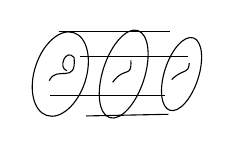
\begin{tikzpicture}[scale=.7]
\draw[rotate around={-18:(0,0)}] (0,0) ellipse (.47 and .79);
\draw[rotate around={-18:(1.15,0)}] (1.15,0) ellipse (.38 and .83);
\draw[rotate around={-18:(2.2,0)}] (2.2,0) ellipse (.31 and .69);
\draw (-.03,.78)--(1.99,.78);
\draw (.36,.32)--(2.32,.32);
\draw (-.18,-.39)--(1.9,-.39);
\draw (.47,-.76)--(1.96,-.73);
\draw (-.20,-.12)..controls (-.07,.17) and (.3,-.2)..(.25,.3)
..controls (.10,.48) and (-.05,.11)..(.12,.06);
\draw (.95,-.15)..controls (1.17,.15) and (1.30,-.08)..(1.28,.25);
\draw (2.02,-.10)..controls (2.25,.12) and (2.32,-.02)..(2.34,.2);
\end{tikzpicture}}}

\uline{Corollaire} \deleted{\unsure{Soit}}
Soit $U$ de type fini sur $k$, $Y$
\deleted{\unsure{quelconque}}
(quelc. sur $k$) \inserted{$y\in Y$}
$R$ un revêtement étale \inserted{gal} de $U\times_k Y$,
de groupe $\Gamma$ premier à $p$.
\deleted{\unsure{Alors $U$}}
Si $R_y$ est un rev. géom trivial,
Alors $R$ est, en dessus d'un voisinage de
\deleted{\unsure{$U(k)$}}
$y$, l'image \unsure{directe|inverse} d'un rev étale d'un tel voisinage.

\uline{Cor.} Soient $X',X''$ propres sur $k$,
$Z'$ ($Z''$) des parties fermées, \deleted{\unsure{alors}} écrivons
\deleted{\unsure{Soit}}
$X=X'\times X''$, $Z=Z'\times X''\cup X'\times Z''$,
enfin considérons les grps
$\pi_1^t(X';Z',x')$, $\pi_1^t(X'';Z'';x'')$ et
$\pi_1^t(X;\deleted{X'\times X''}Z,x)$,
\deleted{Alors} soient $\pi,\pi',\pi''$.
Alors
\[
\deleted{\pi_1^t(X)}\quad \pi\longrightarrow\pi'\times\pi''
\]
est un \uline{\unsure{isomorphisme}}.

\uline{Cor.} Soient $X,Y$ de type fini sur $k$.
Considérons $\pi'_1(X)$ et $\pi'_1(Y)$,
\inserted{$\pi'_1(X\times Y)$}
[rev. étales premiers à la car].
Alors
\[
\pi'_1(X\times Y)\simeq\pi'_1(X)\times\pi'_1(Y).
\]

\scanpage{64}
\mspage{4.}
% archive foliation: 63
\diagram{\begin{tikzcd}
&X'\ \text{normalisé}\arrow[d]&\\
Y\arrow[r,phantom,"\subset" description]&X\text{--}\uline{\text{complet}}&
U=X-Y\\
&\text{réduit}&
\end{tikzcd}}
$Y_1\ldots Y_r$ les composantes de $Y$ de codim $1$ dans $X$

$Y'_{ij}$ les images inverses des $Y_i$ dans $X'$

\deleted{\unsure{Th}}
\deleted{\uline{Th} (1.)\quad$\unsure{\pi_1(U)}$
le quotient de $\pi_1(U)$ par le noyau de
$\pi_1(U)\longrightarrow\pi_1(X)$
est \unsure{un groupe de}}
Considérons les rev. étales de $X-Y$ qui
\deleted{\unsure{y sont définis}}
donnent des rev. \uuline{doux} des $\underline O_{\unsure{Y'_{ij}|Y_{ij}}}$,
ils sont classifiés par un groupe de type profini $\pi$.

\uline{Thm.} Le groupe $\pi$ est top. de génération finie.

\uline{Cor. 1} Soit $X$ \deleted{\unsure{Y}} complet,
$Y$ de codim $>1$, \inserted{$U=X-Y$,}
Alors $\pi_1(\unsure{U}\deleted{\unsure{X-Y}})$
est top. de génération finie.

\uline{Cor 2} Soit $X$ \deleted{de type} alg.
Alors $\pi'_1(X)$ est top. de type fini

\figure{\begin{tikzpicture}[x=1cm,y=1cm]
\draw (0,0)--(1.35,.08); \draw (.15,-.10)--(1.18,-.08);
\draw[->] (2.55,.35)--(2.55,.02);
\draw[->] (5,.27)--(5,-.27);
\draw (2.96,-2.95)--(3.22,-2.58);
\draw (3.02,-2.64)--(3.26,-2.96);
\end{tikzpicture}}

\scanpage{65}
% archive foliation: 64
\diagram{\begin{tikzcd}
\pi_1(X\times Y)\arrow[r,"\uline{\text{surj}}"]&\pi_1(X)\times\pi_1(Y)
\end{tikzcd}}
\figure{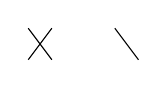
\begin{tikzpicture}\draw (0,0)--(.3,.4);\draw (0,.4)--(.3,0);\draw (1.1,.4)--(1.4,0);\end{tikzpicture}}

\diagram{\begin{tikzcd}
X\arrow[d]&Z\arrow[l,phantom,"\supset" description]\\Y&
\end{tikzcd}}
\diagram{\begin{tikzcd}
\pi_1(\unsure{Z})\arrow[r,no head]&\pi_1(X)\arrow[r,no head]&\pi_1(Y)
\end{tikzcd}}

\diagram{\begin{tikzcd}
X''\arrow[d,shift left=.4ex]\arrow[d,shift right=.4ex]\\
X'\arrow[d]\\X\arrow[d]\\ \cdot
\end{tikzcd}}
\figure{\begin{tikzpicture}
\draw[line width=2pt] (0,0)--(0,1.8);
\draw (-3.3,-1.0)--(-3.65,-.05);
\draw (-3.65,-1.0)--(-3.3,.05);
\fill (-3.48,-.48) circle (.065);
\draw (-2.7,-1.45)..controls (-3,-1.5) and (-2.9,.85)..(-2.72,.82)
..controls (-2.48,.80) and (-2.55,-1.5)..(-2.7,-1.45);
\end{tikzpicture}}

\diagram{\begin{tikzcd}
X\arrow[d]\arrow[r,phantom,"\subset" description]&\widehat X\arrow[d]&\text{normaux}\\
X_0\arrow[r,phantom,"\subset" description]&\widehat X_0&\unsure{\text{pts réguliers}}
\end{tikzcd}}
\figure{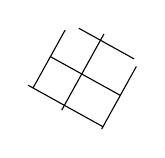
\begin{tikzpicture}[rotate=-29,scale=.7]
\draw (0,0)--(0,1.2); \draw (.65,-.1)--(.65,1.48);
\draw (1.45,-.05)--(1.45,1.25);
\draw (-.1,0)--(1.45,0); \draw (0,.65)--(1.45,.65);
\draw (.2,1.35)--(1.35,1.35);
\end{tikzpicture}}

\diagram{\begin{tikzcd}
Y'\arrow[r,no head]\arrow[d]&X'\arrow[d]\\
Y\arrow[r,phantom,"\subset" description]&X\arrow[d]\\
&P^r
\end{tikzcd}}
\diagram{\begin{tikzcd}
X'\arrow[r,phantom,"\subset" description]\arrow[d]&\unsure{\widehat X'|\overline X'}\arrow[d]\\
X\arrow[r,phantom,"\subset" description]\arrow[d]&\overline X\arrow[dl]\\
P^r&
\end{tikzcd}}
\diagram{\begin{tikzcd}
Y\arrow[r]\arrow[d]&X\arrow[d]\\
H\arrow[r]&P^r\\
/ K&/ k
\end{tikzcd}}
\diagram{\begin{tikzcd}\pi_1(Y)\arrow[r]&\pi_1(X)\end{tikzcd}}
$X$ normal

\diagram{\begin{tikzcd}
\pi_1(Y)\arrow[r,"\text{surj??}"]&\pi_1(X)
\end{tikzcd}}
\[
\pi_1(X)
\]
\figure{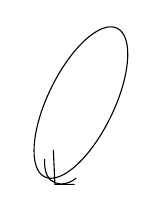
\begin{tikzpicture}
\draw[rotate around={-26:(0,0)}] (0,0) ellipse (.42 and 1.05);
\draw (-.46,-.72)..controls (-.48,-1.07) and (-.22,-1.09)..(-.06,-.96);
\draw (-.35,-.6)--(-.33,-1.04)--(-.08,-1.04);
\end{tikzpicture}}
\deleted{\diagram{\begin{tikzcd}
\pi_1(Y)\arrow[r]&\pi_1(X)&\pi_1(X-Y)\arrow[l]
\end{tikzcd}}}

\scanpage{66}
\mspage{A.}
% archive foliation: 65
\margin{\uline{$\pi_1$ birationnel}}
\uline{Th.} Soient $k$ un corps alg. clos, $X$ schéma
\deleted{propre}\inserted{connexe} sur $k$,
\deleted{$Y$ une partie fermée}
tel que tte composante irréductible $X_i$ soit isomorphe
(pour la structure réduite induite) au
\deleted{\unsure{le complément}}
``complémentaire'' d'une partie fermée de codim $\geq2$ dans un schéma propre
sur $k$. Alors $\pi_1(X)$ est top. de type fini.

\margin{\uline{Question}
Soit $Y\subset X$ fermé, de codim $\geq2$ alors
$\pi_1(X-Y)\to\pi_1(X)$ a un noyau de type fini ???}

Démonstration. Par SGA IX 6.2, on est ramené au cas où
$X$ est \deleted{\uline{irréductible}}\inserted{intègre},
\deleted{et} de la forme $X=Z-Y$, où $Z$ est propre et $Y$ de
codim $\geq2$ dans $Z$.
On aura aussi $X=\overline X-\overline X\cap Y$,
et $\overline X$ est une composante irréductible de $Z$,
$\overline X\cap Y$ y est de codim $\geq2$.
Donc on peut supposer $Z$
\deleted{\unsure{irréductible}}\inserted{intègre},
et on est ramené à prouver le

\uline{Corollaire} $Z$ intègre et propre sur $k$, $Y$ \inserted{fermé} de codim $\geq2$ dans $Z$, $X=Z-Y$,
alors $\pi_1(X)$ est top de type fini.

Soit $Z'\to Z$ un morphisme propre surjectif, avec $Z'$ intègre,
soit $X'$ l'image inverse de $X$ dans $Z'$,
on a $X'=Z'-Y'$, et $Y'$ de codim $\geq2$
\inserted{dans $Z'$}.
Par loc cit. il suffit de prouver que $\pi_1(X')$ est top.
de type fini. Par le \uline{lemme de Chow},

\scanpage{67}
\mspage{B.}
% archive foliation: 66
on peut donc supposer que $Z$ est \uline{projectif},
\deleted{Si dim} et $=$ \uline{normal} si on veut.
Si \inserted{$\dim Z\leq0$, trivial. Si}
$\dim Z=1$, on aura $Y=\varnothing$, i.e. $X=Z$,
et le th. est connu. Si $\dim Z\geq2$ on utilise ceci:

\uline{Lemme} de \uline{Bertini} (Zariski)
Soit $k$ corps,
$X\xrightarrow{f}\unsure{\mathbf P|P}_k^r$ un \uline{morphisme},
avec $X$ \uline{irréductible},
$\dim f(X)\unsure{=|\geq}n$, soit $1\leq s\leq n-1$, et soit $u$
le point générique de
$\underbrace{\unsure{\mathbf P|P}_k^r\times\cdots\times\unsure{\mathbf P|P}_k^r}_{s}$,
et $K$ une clôture algébrique de $k(u)$,
enfin $L_u$ la variété linéaire de $\unsure{\mathbf P|P}_K^r$ définie par $u$,
et
\[
X_u=X\times_{\unsure{\mathbf P|P}_k^r}L_u=X_K\times_{\unsure{\mathbf P|P}_K^r}L_u.
\]
Alors $X_u$ est irréductible.

\margin{peut-on remplacer ``irréductible'' par ``connexe'' ?
\uline{non}}

\margin{\diagram{\begin{tikzcd}
X'_u\arrow[d]&&X'\arrow[d]\\
X_u\arrow[r]\arrow[d]&X_K\arrow[r]\arrow[d]&X\arrow[d]\\
L_u\arrow[r]&\unsure{\mathbf P|P}_K^r\arrow[r]&\unsure{\mathbf P|P}_k^r
\end{tikzcd}}}

\uline{Corollaire} \deleted{\unsure{Soit}}
Si $X$ est \uline{normal}, alors
$\pi_1(X_u)\to\pi_1(X)$ est \uline{surjectif}.

En effet, si $X'$ est un revêtement \deleted{normal}
étale connexe de $X$, étant normal il est \uline{irréductible},
donc $X'_u=X'\times_X X_u$ est irréductible,
donc connexe, OK.

\margin{Si on admet le th. de connexion,
on \deleted{peut} \unsure{pourra alors} utiliser une
\unsure{section}
\deleted{\unsure{pas}}
``\unsure{spéciale}'' \ldots\ pour une courbe.}

\scanpage{68}
\mspage{C}
% archive foliation: 67
Reprenons notre $Z$ normal de dim $n\geq2$, et $X=Z-Y$.
Plongeons $Z$ dans $P^r$, et le morphisme induit $f:X\to P^r$.
On prend $s=n-1$, de sorte que
$X_u$ \deleted{est une \uline{courbe}}
\inserted{$=X_K\cap L_u=Z_K\cap L_u$, car $Y_K\cap L_u=\varnothing$,}
donc $X_u=Z_K\cap L_u$ est une \uline{courbe} de
\deleted{genre $g$} projective, d'ailleurs normale.
Si $g$ est son genre, il résulte alors du corollaire au lemme de Bertini
que $\pi_1(X)$ admet $2g$ générateurs topologiques, OK.

\uline{Conséquence.} Soit $K$ une extension de type fini d'un corps $k$.
Il existe tjrs des modèles projectifs,
\deleted{\unsure{(Alors normaux}}
à fortiori propres, et normaux si on veut,
\deleted{donc réguliers en codim $\leq1$,}
\deleted{\inserted{Soit $X$ \unsure{le}}
\unsure{les modèles de tels}}
\deleted{modèles réguliers $U$ qui sont
\unsure{gros}
``\uline{presque propres}'', i.e. complémentaires
d'un ens fermé de codim $\geq2$ dans un modèle propre $X$.
D'ailleurs, tts les modèles $U$ comme dessus, ordonnés par}

\margin{\diagram{\begin{tikzcd}
&X''\arrow[dl,no head]\arrow[dr,no head]&\\
X&&X'
\end{tikzcd}}}

\scanpage{69}
\mspage{D}
% archive foliation: 68
D'ailleurs les modèles propres et normaux, pour la relation de domination,
forment un ordonné \uline{filtrant croissant},
\deleted{\unsure{on a}}
Soit $U_0$ un \deleted{tel} modèle
\deleted{\unsure{de l'un des ens pts réguliers}}
\inserted{régulier de $K$},
et soit $X_{\unsure{1|\alpha}}$
\deleted{dominant $X_0$}
\inserted{propre \deleted{\unsure{normal}} \uline{dominant}}.

\margin{\diagram{\begin{tikzcd}
&X''&\\
\deleted{\unsure{U}}X\arrow[ur,no head]\arrow[r,no head]&X'\deleted{\unsure{U'}}&
\end{tikzcd}}}

\deleted{Soit $\unsure{U_1|U_0}$ \unsure{l'ens des pts} de $U_0$ où
l'application rationnelle évidente \deleted{\unsure{$X$}}
$U_0\to X_{\unsure{1|\alpha}}$ induit
\deleted{\unsure{par $f$}} est définie,
c'est \inserted{le compl. du lieu d'}
\unsure{un ens fermé} de codim $\geq2$,
\deleted{\unsure{donc d'après le}}
et on a donc
\deleted{complémentaire dans $X_0$ d'un ens fermé de codim $\geq2$.}
\unsure{On a un}
\deleted{\unsure{hom canonique}},
diagramme commutatif, donc on voit que on a un hom surjectif}

\margin{\diagram{\begin{tikzcd}
X_{\unsure{1|\alpha}}\arrow[d,"f"']&&\\
X_0\arrow[r,phantom,"\supset" description]&
U_0\arrow[r,phantom,"\supset" description]&
U_{\unsure{1|\alpha}}\arrow[ull,"g"']
\end{tikzcd}}}
\margin{\diagram{\begin{tikzcd}
\pi_1(X_{\unsure{1|\alpha}})\arrow[dd,"f_*"']&
\deleted{\pi_1(U_{\unsure{1|\alpha}})}\arrow[l]&\\
&&\\
\pi_1(X_0)&\pi_1(U_0)\arrow[l]&
\pi_1(U_1)\arrow[l,"\simeq" above,"\text{th. de pureté}" below]\arrow[uull,"g_*"]
\end{tikzcd}}}

L'application rationnelle évidente $U\to X$ est définie sur le
complémentaire d'une partie fermée de codim $\geq2$,
on voit que (par le th. de pureté) on en tire un hom
\uline{surjectif} (car $X$ normal)
\[
\pi_1(U)\longrightarrow\pi_1(X)
\]
d'où à la limite un hom \uuline{surjectif}
\[
\pi_1(U;\Omega)\longrightarrow
\varprojlim_{\substack{X\ \text{modèle}\\\text{propre}}}
\pi_1(X;\Omega)
\]
où $\Omega$ est une extension alg. close de $K$.

\margin{\deleted{\unsure{of}}}

\scanpage{70}
\mspage{E.}
% archive foliation: 69
Le dernier \unsure{est} est appelé le \uline{groupe fondamental birationnel}
de $K/k$.
[N.B. il y aurait à l'introduire plutôt comme groupe alg. \unsure{lié|lin}
sur $K$],
\inserted{noté $\pi_1(K/k;\Omega)$.}
\inserted{Pour tt modèle propre \uline{projectif} $X$,
$\pi_1(X;\Omega)$ est un quotient de $\pi_1(K/k;\Omega)$.}
On voit donc qu'il est, de plus, un quotient de $\pi_1(U)$.
Donc, comme
\inserted{$U$ peut être pris complémentaire d'une partie fermée de codim $\geq2$
dans un schéma intègre propre;}
\uline{Th.} Si $K/k$ est une extension de type fini avec $k$ alg. clos,
alors
\deleted{\unsure{Alors}}
$\pi_1(K/k;\Omega)$ est top$ {}^t$ de type fini.

\margin{\uline{Remarque}
Si $K$ a un modèle propre régulier, alors pour $X'$ propre normal
dominant $X$, on a
$\pi_1(X;\Omega)\simeq\pi_1(X';\Omega)$,
donc le système projectif des $\pi_1(X_i;\Omega)$,
$X_i$ propre normal, est essentiellement constant.
Qu'en est-il en général ??? Si $X$ est un modèle propre normal,
\deleted{\unsure{tout}}
$U$ l'ouv de ses pts réguliers, est-il vrai que
$\pi_1(U;\Omega)\to\pi_1(K/k;\Omega)$ est bijectif,
i.e. que tte
\deleted{\unsure{modèle $X$}}
extension finie $K'$ de $K$,
non ramifiée sur $U$, est non ramifiée
sur un modèle $X'$ \unsure{déduit de}
$X$ \unsure{par éclatemts} ?
C'est une question au fond de \unsure{schémas génériques} \ldots}

\scanpage{71}
\mspage{F.}
% archive foliation: 70
\margin{\uline{Pic birationnel}}
\uline{Théorème} Soient $f:X\to Y$ un morphisme \inserted{birationnel} dominant
de préschémas intègres normaux \deleted{et} propres sur $k$,
avec $Y$ \deleted{factoriel}\inserted{\deleted{\unsure{loc.}}\uline{régulier}}.
Alors le morphisme
\[
\underline{\mathrm{Pic}}_Y^\tau\longrightarrow
\underline{\mathrm{Pic}}_X^\tau
\]
est un \uline{isomorphisme}.

\margin{$X$ normal ``sur $k$'' ?}
\margin{peut-on \deleted{\unsure{supposer $Y$ régulier??}}
\deleted{\unsure{connexe}} \unsure{sur $k$} ?}
\margin{N.B. factoriel ne suffit pas $=$ \unsure{est des pts de ces}
\unsure{non-réduits, cf côtés} \ldots}

C'est un \uline{monomorphisme} grâce au fait que
$f_*(\underline O_X)=\underline O_Y$ (universellement sur $k$ !),
donc une immersion fermée puisque un hom de groupes
\unsure{-- en principe} propre.
Montrons que c'est \uline{surjectif}.
Soit $U$ l'ouv de $Y$ où $f^{-1}$ est défini,
comme $Y$ est factoriel, on a
\[
\mathrm{Pic}(X)\xrightarrow{\simeq}\mathrm{Pic}(U),
\]
d'où, utilisant
\diagram{\begin{tikzcd}
&X\arrow[d,"f"]\\
U\arrow[ur,"g"]\arrow[r,"i"']&Y
\end{tikzcd}},
le diagramme commutatif
\diagram{\begin{tikzcd}
&\mathrm{Pic}(X)\arrow[dl,leftrightarrow,"g^*"']\\
\mathrm{Pic}(U)&\mathrm{Pic}(Y)\arrow[l,"\simeq","i^*"']\arrow[u,"f^*"']
\end{tikzcd}}
qui montre que $\mathrm{Pic}(Y)\to\mathrm{Pic}(X)$ est un hom
sur un facteur direct, l'image étant formée des $\xi$ telles que
\deleted{$g^*(\xi)=0$.}
$\xi=f^*i^{*-1}g^*(\xi)$.
Or si $\xi$ est \deleted{\unsure{même}} $\tau$-équivalente à $0$,
\inserted{donc $\eta=m\xi$ est alg. équiv. à $0$,}
\deleted{\unsure{alors}}
$g^*(\unsure{\eta|\xi})$ est
\deleted{$\tau$-équivalente}\inserted{alg. équiv.} à $0$,
donc $i^{*-1}g^*(\unsure{\eta|\xi})\deleted{\text{\unsure{même}}}$ aussi,
donc $mf^*i^{*-1}g^*(\xi)$
\inserted{$=mf^*(i^{*-1}g^*(\xi))$}
\deleted{\unsure{aussi}}.
D'autre part, on voit que
\inserted{$\xi-f^*i^{*-1}g^*(\xi)$}
\deleted{\unsure{le diviseur exceptionnel}}
est représenté par un

\margin{\figure{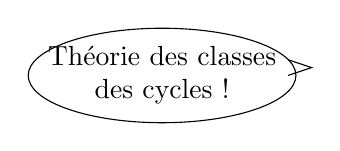
\begin{tikzpicture}\draw (0,0) ellipse (1.7 and .6);\draw (1.6,.2)--(1.9,.1)--(1.6,0);\node[align=center] at (0,0) {Théorie des \unsure{classes}\\des cycles !};\end{tikzpicture}}}
\margin{$Y$ projectif ?? ou \unsure{proj.} sur $k$}

\scanpage{72}
\mspage{G.}
% archive foliation: 71
diviseur $\sum n_iX_i$, où les $X_i$ sont les ``diviseurs singuliers''
pour $f$. Il reste donc à voir que si une telle combinaison linéaire est
\deleted{algébriquement}
$\tau$-équivalente à $0$, elle est nulle.
\deleted{\unsure{Or}}
C'est là un lemme bien connu \ldots

\margin{vérifier ? On peut se ramener au cas projectif}
\margin{\uline{insuffisant}}

Ainsi, $f:\underline{\mathrm{Pic}}_Y^\tau\mathbin{\unsure{-|\longrightarrow}}
\underline{\mathrm{Pic}}_X^\tau$ est une \uline{immersion}
\uline{surjective}.
Il \uline{reste à prouver} qu'elle induit un isom sur les espaces tangents
à l'origine, donc à vérifier le

\uline{Corollaire} Sous les conditions du th., l'homomorphisme
\[
f^*:H^1(Y,\underline O_Y)\longrightarrow H^1(X,\underline O_X)
\]
est un isomorphisme.

On sait déjà que c'est injectif, la question est la surjectivité.
\deleted{En effet}
En caractéristique $p>0$, il suffit de prouver qu'on a bijectivité
\[
H^1(Y,\underline O_Y)^F
\mathbin{\unsure{-|\longrightarrow}}
H^1(X,\underline O_X)^F
\]
\[
{}_{F^{\unsure{\nu|1}}}H^1(Y,\underline O_Y)
\mathbin{\unsure{-|\longrightarrow}}
{}_{F^{\unsure{\nu|1}}}H^1(X,\underline O_X)
\]
où $F$ est le Frobenius.
Le premier hom s'écrit
\[
H^1(Y,\mathbf Z/p\mathbf Z)\longrightarrow H^1(X,\mathbf Z/p\mathbf Z)
\]

\scanpage{73}
\mspage{H}
\deleted{\unsure{H}}
% archive foliation: 72
c'est un isomorphisme à cause du fait que
$\pi_1(X)\mathbin{\unsure{-|\to}}\pi_1(Y)$ est un isomorphisme
[grâce au th. de pureté sur $Y$]
\margin{$Y$ \uline{régulier}}

Le deuxième homomorphisme s'écrit
\[
H^0(Y,\underline O_Y/\underline O_Y^{p^{\unsure{\nu|1}}})
\longrightarrow
H^0(X,\underline O_X/\underline O_X^{p^{\unsure{\nu|1}}})
\]
[grâce au fait que $X,Y$ sont réduits],
ou aussi, supposant que $k$ est alg. clos donc parfait,
s'interprète comme
\[
f^*:H^0(Y,\underline O_Y^{p^{-\unsure{\nu|1}}}/\underline O_Y)
\longrightarrow
H^0(X,\underline O_X^{p^{-\unsure{\nu|1}}}/\underline O_X)
\]
\margin{$Y$ \unsure{lisse} sur $k$ (!)}

Ce dernier est bijectif grâce à la \uline{normalité} de $X$ et $Y$,
car \deleted{\unsure{si $f$}} avec les notations ci-dessus, on a un
diagramme commutatif
\diagram{\begin{tikzcd}
&T(X)\arrow[dl,"g^*"']\\
T(U)&T(Y)\arrow[l,"\simeq","i^*"']\arrow[u,"f^*"']
\end{tikzcd}}
avec $g^*$ \uline{injective}
[car $\underline O_X^{p^{-\unsure{\nu|1}}}/
\underline O_X^{\unsure{\tau}}$ est \deleted{\unsure{li}}
sans \uline{torsion} \ldots],
d'où $f^*$ et $i^{*-1}g^*$ sont des isom inverses l'un de l'autre.
\margin{$X$ \uline{normal}}

\scanpage{74}
\mspage{I}
% archive foliation: 73
Dans le cas où $k$ est de car. $0$, on peut supposer que $k$ est
\deleted{de type fini sur $\mathbf Q$}
le corps des fractions d'un schéma intègre $S$ de type fini sur $\mathbf Z$,
et que $f:X\mathbin{\unsure{-|\to}}Y$ provient d'un morphisme de
$S$-préschémas $\overline f:\overline X\mathbin{\unsure{-|\to}}\overline Y$,
intègres, $\overline Y$ simple sur $S$, et $\overline X$
\deleted{simple} normal sur $S$, les fibres de l'un et l'autre étant
\unsure{géomt} connexes.
\deleted{Alors \unsure{pour}
$\forall\,\unsure{y\in Y|s\in S}$ \unsure{sc}
$H^1(Y,\underline O_Y)\to H^1(X,\underline O_X)$
est de dim $r$, il existe un
\unsure{peut supposer qu'il est constant}.}
On peut supposer aussi $X$ et $Y$ coh. plats sur $S$ en dim $1$,
\deleted{\unsure{enfin que}}
Alors \deleted{\unsure{celui}}
l'hom
$R^1q_*(\underline O_{\overline Y})\mathbin{\unsure{-|\to}}
R^1p_*(\underline O_{\overline X})$
est injectif, \deleted{et que}
(car il l'est en tt pt par \unsure{évidence|réduction}).
Alors \unsure{rétrécissant} $S$, si le \unsure{conoyau}
du $H^1(Y,\underline O_Y)\mathbin{-}H^1(X,\underline O_X)$
est de dim $r$, la $=$ chose sera vraie pour les fibres en \uline{tous}
les points $s\in S$, en particulier en des pts de

\scanpage{75}
\mspage{J}
% archive foliation: 74
car $>0$. Cela prouve $r=0$, et achève la démonstration.

\uline{Corollaire 1} Invariance birationnelle de $\uline{\mathrm{Pic}}^\tau_{X/k}$
pour $X$ propre et simple sur $k$.

\uline{Corollaire 2} Soit $K$ une extension
\deleted{régulière}\inserted{\unsure{séparable primaire|séparablement primaire}}
de type fini de $k$, admettant un modèle \deleted{régulier}
propre et \uline{simple} sur $k$. Alors
$\varinjlim_X\uline{\mathrm{Pic}}^\tau_{X/k}$, où $X$ parcourt
les modèles propres et normaux \inserted{``sur $k$''} de $K$
existe au sens usuel [le système \deleted{projectif}\inserted{inductif}
est essentiellement constant].

\margin{\uline{N.B.} Si $k$ n'est pas parfait, et $K$ est de dim $1$ sur $k$,
\deleted{\unsure{donc}} c'est une condition un peu idiote!}

\uline{Question}. Le cor. 2 reste-t-il valable
en supposant seulement que $K$ admette
un modèle ``normal sur $k$''??
\deleted{\unsure{Il y aurait}}\inserted{\unsure{Cela}}
\deleted{\unsure{du moins}} équivaudrait à la conjonction des
assertions suivantes
\[
\begin{array}{ll}
\text{(i)}&\dim\uline{\mathrm{Pic}}_{X/k}\text{ reste majoré}\\
\text{(ii)}&\text{ordre }\boxed{\mathrm{Tors}\,\uline{\mathrm{Pic}}(X/k)}
                    \text{ reste majoré}\\
\text{(iii)}&\dim\boxed{H^1(X,\underline O_X)}\text{ reste majoré.}
\end{array}
\]
\margin{N.B. (i) résulte de (iii)}

\scanpage{76}
\mspage{K}
% archive foliation: 75
\uline{Théorème} Soit $K$ une extension de type fini du
corps $k$, \deleted{[ayant au moins un modèle
propre \inserted{\unsure{sur $k$|sur}} et universellement normal sur $k$]}
\deleted{Soit} Il
\deleted{$(X_i)_{i\in I}$ le système \unsure{ind}}
existe un entier $n(K/k)$
tel que pour tout modèle \inserted{$X$ de $K$} propre sur $k$, et
normal sur $k$, \deleted{\unsure{pour}} on ait \deleted{$\dim\uline{\mathrm{Pic}}_X$}
\[
\dim\uline{\mathrm{Pic}}_{X/k}\leq n(K/k)
\]

\uline{Démonstration}. \deleted{\unsure{On est ramené au cas}}
\inserted{S'il n'existe pas de}
modèle $X$ du type indiqué, c'est trivial.
Sinon $K$ est séparable sur $k$, et
$\overline K=K\otimes_k\overline k$ est une extension de type
fini du corps alg. clos $\overline k$, et on
est ramené au cas où $k$ est alg. clos.
Alors
\[
\dim\uline{\mathrm{Pic}}_{X/k}
=\tfrac12\operatorname{rang}_{\mathbf Z_\ell}
(\text{partie $\ell$-primaire de }\pi_1(X/k)\text{ rendu abélien})
\]
et à ce titre, \unsure{on renvoie aux} théorèmes
de majoration uniforme des $\pi_1(X/k)$

\scanpage{77}
\mspage{L}
% archive foliation: 76
pour les modèles normaux (\unsure{résultant} de
la partie facile de Lefschetz, du moins pour
les groupes fondamentaux rendus abéliens),
on a fini. De façon plus précise
il suffit, pour un \inserted{modèle} $X$ \uline{projectif} sur $k$,
(propre et normal), de prendre dans $X$
une ``courbe générique $C$'' et pour
$n(K)$ le genre de la dite courbe
générique.

\margin{\diagram{
\begin{tikzcd}
C' \arrow[r,phantom,"\subset"] \arrow[d] & X' \arrow[d] & \\
C_{k(\unsure{u|\omega})} \arrow[r,phantom,"\subset"] & X \arrow[r,phantom,"\subset"] & P^r
\end{tikzcd}
}}

Y-a-t-il une démonstration du fait
que cela donne une majoration, n'utilisant
pas la théorie du groupe fondamental
et le fait que $\uline{\mathrm{Pic}}^\tau_{X/k}$ est propre sur $k$
si $X$ est normale?
\margin{démonstration directe???}

\scanpage{78}
% archive foliation: 77
\deleted{Comparaison d'un
anneau hensélien
et son complété
($\pi_1$, \unsure{faisc. ét...})}

\uline{Revêtements formels}

\uline{étales}

\uline{et th. de Mumford}

\scanpage{82}
% archive foliation: 81
\[
\begin{array}{c|l}
\mathrm I&3\\
&7\ \unsure{\leftarrow}\ 9\\
&11\\
&12
\end{array}
\]
\margin{\unsure{total to} \unsure{all the} \unsure{implications}}
\margin{\fbox{\parbox{5cm}{ambiguity on points of formal schemes
quite general ---}}}

\deleted{\unsure{18|13} --- Most examples come from usual
\unsure{proper} schemes over $\mathbf Z$!}
\[
\begin{array}{l}
20\\27
\end{array}
\]

whole chapter looks plethoric

\[
\begin{array}{ll}
\mathrm{II}&2\\
&12\quad\text{unreasonable!}\\
&16\\&20\\&22
\end{array}
\]

\diagram{
\begin{tikzcd}[column sep=small,row sep=large]
& \boxed{\parbox{9cm}{explicit interpretation of $\pi_1^D$ in terms of
$\unsure{\mathfrak S}-\unsure{\operatorname{Supp}|\operatorname{Spec}}\,D$}}
\arrow[dl,leftrightarrow]\\
\boxed{\parbox{4cm}{whole chapter III seems to be used only to get
$\boxed{3.5.8}$}} &
\end{tikzcd}
}
\fbox{\parbox{10cm}{Copy of previous note on tame ramification?}}

\fbox{\parbox{10cm}{Include variant of Lefschetz's Theorem for $\pi_1^t$}}

\fbox{\parbox{10cm}{Include, after Mumford's theorem,
application to question of finite generation of local
\deleted{tame}\inserted{prime to $p$ ---} fund. group.}}

\[
\begin{array}{ll}
\underline{\mathrm{III}}&\underline{1}\\&2\\&6\quad\text{2 fois}\\&8\\&11\\&12^b
\end{array}
\]

16\quad add section on case when D.'s have equations!
This should make the situation much clearer!
For instance 3.4.1, 3.4.2

22

25\quad fppf descent for tamely ramified coverings?
At least one would like to have a ``champ'' on $\mathrm{Et}/S$!

26\quad \unsure{a)}\\
\hspace*{2em}\unsure{b)} Normality assumption more natural
(formal normality, \unsure{in loc.} formal schemes---)

28\quad\unsure{15}

\margin{cf 3.6.4}

Proof of $3.6.\unsure{5|8}$ is unbelievably long!

\figure{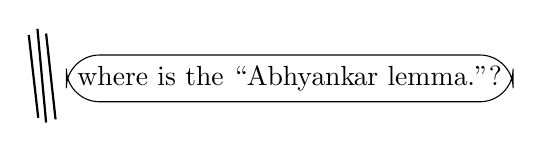
\begin{tikzpicture}[x=1cm,y=1cm]
\draw[line width=.8pt] (0,0)--(-.12,1.05) (.10,-.06)--(-.01,1.13) (.22,-.02)--(.10,1.07);
\node[draw,rounded corners=12pt,anchor=west,inner sep=4pt] at (.35,.5) {where is the ``Abhyankar lemma.''?};
\end{tikzpicture}}

\scanpage{84}
% archive foliation: 83
\uline{IV}\quad \unsure{4.1.2}\quad
4.1.2 \unsure{trivial} in terms of \uline{III} p. 16 added.

Quite \inserted{\unsure{for $s^*$}} cumbersome; take point of
$\operatorname{Spec}(\underline O_{S,s})$!

6\quad Introduce geometric points of $S$.

\uline{VI}\quad 2\quad\unsure{inutile}

7\quad What is the meaning?

$\left.\begin{array}{l}9\\11\end{array}\right\}$
6.1.1 and 6.2.2 could be made into a single example!

\margin{\figure{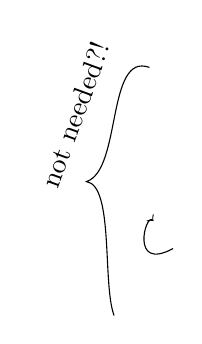
\begin{tikzpicture}[x=1cm,y=1cm]
\draw (1,3.4) .. controls (.45,3.6) and (.65,2.1) .. (.20,1.95) .. controls (.55,1.90) and (.40,.65) .. (.55,.25);
\node[rotate=70] at (.05,2.8) {not needed?!};
\draw[->] (1.3,1.1) .. controls (.75,.8) and (.95,1.55) .. (1.05,1.45);
\end{tikzpicture}}}

VII\quad 1

2\quad I guess that one has equivalence of categories anyhow!!

\margin{\figure{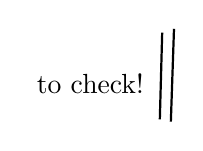
\begin{tikzpicture}[x=1cm,y=1cm]
\node[anchor=east] at (0,.45) {to check!};
\draw[line width=.8pt] (.08,0)--(.11,1.1) (.22,-.03)--(.26,1.15);
\end{tikzpicture}}}

9

\uline{VIII}\quad 1\\
\hspace*{3em}2

$3/\unsure{8.1.6|8.1.1}$ Not too clear. Say that if
\deleted{$A$ a local or \deleted{\unsure{local}} henselian ring, then to any}
\inserted{$S$ any scheme}
(for instance the localization of $S$ at $s_0$)
and \deleted{$s_0,s_0^*$ two points,}
$x,y$ two points, $x\in\overline{\{y\}}$,
\deleted{then the} with, given just geom. $\bar x,\bar y$
$\overline{k(x)}/x$, $\overline{k(y)}/y$, then the ``paths'' of $\bar y$ to $\bar x$
\deleted{$\unsure{\bar x},\bar y$}
correspond exactly to the \deleted{point} liftings
i.e. to the \inserted{$k(y)$-}hom of
\[
\operatorname{ring}(\overline S\otimes_S y)=\prod K_i
\quad\text{into }\overline{k(y)}.
\]
\diagram{
\begin{tikzcd}
{\overline S=\text{strict loc. of $S$ at $\bar x$}}\arrow[d]
& \bar y^{\unsure{\prime}}\arrow[l,dashed]\arrow[dl]\\
S&
\end{tikzcd}
}

\uuline{IX}\quad
$\begin{array}{ll}
1&14\ \deleted{\unsure{et}}\\
4&\\
5,6&\\
9&\\
10'&18\\
10''&19\\
12&
\end{array}$

$9.3.4\Rightarrow9.3.5$\quad looks tautological

$9.3.5\Rightarrow9.3.2$\quad very cumbersome!

\margin{yoga \unsure{stemming} from Abhyankar lemma to be used...}

\scanpage{85}
% handwritten top number: 69; attribution of this pagination is uncertain, not asserted as autograph pagination
% archive foliation: 84
\deleted{
Appliquons \deleted{\unsure{8}}7.2.1 \deleted{\unsure{4}} au groupe formel
$\widehat A$, dans le cas favorable
envisagé dans \deleted{\unsure{10}} 7.1 où le schéma
\deleted{\unsure{dit}} formel abélien $\widehat B$ est algébrisable,
\inserted{et où on suppose de plus \deleted{\unsure{que}} $T_0$ isotrivial.}
On trouve alors une \deleted{extension canonique du} schéma
\deleted{abélien B dont le}\inserted{en groupes $A^{\unsure{\natural|\sharp}}$ sur $S$},
\inserted{appelé le \uline{groupe de Raynaud} associé au schéma en groupes $A$ sur $S$,
tel que $A$}
complété formel est $\widehat B$, par le tore $T$ sur $S$ qui remonte $T_0$,
\deleted{\unsure{;}} que nous
appellerons l'\uline{extension de Raynaud} associée à $A$, et que nous noterons
$A^{\unsure{\natural|\sharp}}$ :
\[
(\deleted{\unsure{8}}7.2.2)\qquad
0\longrightarrow T\longrightarrow A^{\unsure{\natural|\sharp}}
\longrightarrow B\longrightarrow0.
\]
Elle est donc définie, à isomorphisme unique près, par le fait qu'elle
donne naissance à un système cohérent d'isomorphismes d'extensions
\[
(7.2.3)\qquad A^{\unsure{\natural|\sharp}}_n\simeq A_n
\]
(le deuxième membre muni de sa structure d'extension décrite dans (7.1.1)
i.e. qu'on a un isomorphisme de \inserted{schémas formels en} groupes
\deleted{formels}
\[
(7.\unsure{2|3}.4)\qquad (A^{\unsure{\natural|\sharp}})^\wedge\simeq\widehat A,
\]
respectant d'ailleurs les structures d'extensions.
\deleted{Il résulte de plus de 7.2.1}

7.2.5. Il résulte d'autre part \deleted{que la} immédiatement de 7.2.1 que la
suite exacte (7.2.2) dépend fonctoriellement du schéma
\inserted{en groupes} $A$ sur $S$ satisfaisant aux conditions envisagées dans 7.1,
et que sa formation commute à
tout changement de base par un homomorphisme $S'\longrightarrow S$
associé à un homomorphisme d'anneaux topologiques noethériens adiques
$V\longrightarrow V'$.
}

\scanpage{86}
% archive foliation: 85
X\quad 1\qquad exists (and is unique) in quasi coherent case.
State that $\mathcal E$ is of finite type (resp. finite
presentation \inserted{or loc. free}) iff $\mathcal E_1,\mathcal E_2$ are.

\margin{\unsure{d}}
5
\margin{$\unsure{+S_3}$}
\figure{
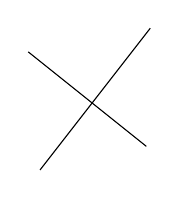
\begin{tikzpicture}
\draw (0,1.5)--(1.5,0.3);
\draw (0.15,0)--(1.55,1.8);
\end{tikzpicture}
}

12\quad Amounts to showing: \deleted{\unsure{$X$}}
\unsure{fnt|finite} flat covering of $S$
is tame with r. to $D_1,D_2$ iff it \deleted{\unsure{is so}}
restriction to $S_1,S_2$ are tamely ramified.
\uline{Should be trivial} with the conditions considered!

\scanpage{87}
% archive foliation: 86
\deleted{
Voyons alors le critère d'\uline{image inverse des
$\mathcal O$-Modules}. Un $\mathcal O$-Module quasi-cohérent
est toujours un $\unsure{\mathrm{Ab}|\mathcal A}$, donc
\uline{Module \inserted{qu. coh.} stratifié} est toujours un \unsure{itou}.
Il faut vérifier que c'est le critère
\unsure{induit|usuel} d'image inverse des Modules
stratifiés.

\medskip\hrule\medskip

Supposons que si $X'\unsure{-|\longrightarrow}X\times_S S'$ est
un \unsure{m.u.} (resp. fini \deleted{\unsure{ou}} non ramifié)
alors le morphisme
$T_0\times_X X'\unsure{-|\longrightarrow}T\times_S S'$
est également un \unsure{m.u.}
(resp. non ramifié)
et peut être muni
de la famille des
voisinages infinitésimaux
de tous ordres,
\unsure{dans le 1er cas}. Alors
\[
f^*(\mathcal F)=\varinjlim_n\mathcal F'_n
\]
\unsure{(comme au dessus)} si $F'$ est un faisceau

\diagram{
\begin{tikzcd}[column sep=small,row sep=large]
& T_0\arrow[dl]\arrow[dd,"\rho"] && T_0\times_S S'\arrow[ll]\arrow[dl,no head]\arrow[dd,"\rho"] &\\
X\arrow[dd] && X\times_S S'\arrow[ll]\arrow[ddd] &&
{T_0\times_X X'=T'_0}\arrow[ul,"\mathrm{n.r.}"']\arrow[dl]\arrow[ddl,dashed,"\mathrm{n.r.}"]\\
& T\arrow[dl] && \deleted{X'}\arrow[ul]\arrow[d]\arrow[ddl,very thick,"\mathrm{n.r.}"'] &\\
S &&& {T\times_S S'\ \unsure{=}\ T'}\arrow[ull,dashed]\arrow[dl,double] &\\
&& S'\arrow[ull] &&
\end{tikzcd}
}
}

\scanpage{88}
\mspage{1}
% archive foliation: 87
$\mathfrak X$ schéma formel régulier, \inserted{connexe},
$\mathfrak X_0=X_0$ diviseur régulier,
$D=\deleted{\unsure{+}}\bigcup_0^{\unsure{r}}D_i$,
\unsure{diviseurs} \deleted{avec} \unsure{normaux}
croisant normalement $D_0=X_0$,
[les $D_i$ réguliers irréductibles]
$D'=\sum_{i\ne0}D_i$, $\unsure{D'_0|D_0}$ induit sur $X_0$.

\diagram{
\begin{tikzcd}[column sep=small]
e\arrow[r]&\overline I_0\arrow[r]&
\pi_1^t(\mathfrak X/D,\bar\xi_1)\arrow[r]&
\pi_1^t(X_0/D'_0,\bar\xi_0)\arrow[r]&e\\
&&\text{''}&\text{''}\quad\text{''}&\\
&&\pi_1^t(\mathfrak X/D)&
\pi_1^t(U)\quad\pi_1(\mathfrak X/D',\bar\xi_0)&\\
&&&\text{''}&\\
&&&D_0-D'_0&
\end{tikzcd}
}
\margin{\figure{
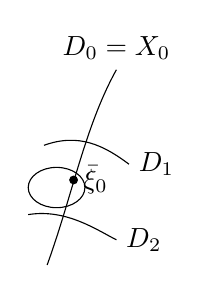
\begin{tikzpicture}[scale=.8]
\draw (0,0) .. controls (.4,1.1) and (.6,2.2) .. (1.1,3.1)
 node[above]{$D_0=X_0$};
\draw (-.05,1.9)..controls(.5,2.1)and(.9,1.9)..(1.3,1.6)node[right]{$D_1$};
\draw (-.3,.8)..controls(.3,.9)and(.8,.55)..(1.1,.4)node[right]{$D_2$};
\fill (.42,1.35)circle(2pt);
\node[right]at(.42,1.35){$\bar\xi_0$};
\draw (.15,1.23)ellipse(.45 and .32);
\end{tikzpicture}
}}

\[
\deleted{\unsure{\mu}\longrightarrow}
\mu^\infty_{X_0,\mathrm{tame}}(\bar\xi_0)
\longrightarrow I_0\longrightarrow0
\]
\[
\begin{array}{c}
\text{''}\\[-2pt]
\mu(\deleted{\unsure{\bar\xi}}\bar\xi_0)
\end{array}
\]
\margin{$=\varprojlim_{\substack{n>0\\n\text{ inversible dans }\underline O_{X_0}}}\mu_n$}

\margin{\diagram{
\begin{tikzcd}
\mu\arrow[r]&I\arrow[r]&0\\
\mu^\infty_{X_0,\mathrm{tame}}\arrow[u,phantom,"\text{''}"]&&
\end{tikzcd}
}
faisceaux étales sur $X_0$}

Donc
\[
\prod_{\ell\underline O_{X_0}=\underline O_{X_0}}\mathbf Z_\ell
\]
\[
\mu(\bar\xi_0)\longrightarrow\pi_1^t(\mathfrak X/D)
\longrightarrow\pi_1^t(U)\longrightarrow e
\]
Opérations de $\pi_1^t(U)$ sur $I_0$ via opérations de
$\pi_1^t(U)$ sur \deleted{$I$}$\mu$
\deleted{\unsure{via op---}}.
L'extension décrite par
\[
\alpha\deleted{\unsure{\xi}}\in H^2(\pi_1^t(U),I_0)
\qquad
\deleted{\unsure{\xi}}\alpha=?
\]

\uline{Lemme 1} Soit $\widetilde U^t$ rev. étale de $U$ défini par
$\pi_1^t$. Alors
\[
H^1(\widetilde U^t,J)=0
\quad\text{si }J\text{ premier aux car. résiduelles de }X_0
\]
[p. ex. $J=I$].
\margin{constant}
\margin{for all $H^i$, $i>0$, true if $D_0$ is \uline{curve}
\uline{over a field}}

\diagram{
\begin{tikzcd}[column sep=small]
0\arrow[r]&H^2(\pi_1^t,I)\arrow[r,"\rho"]&
H^2(U,I)\arrow[r]&
H^2(\widetilde U^t,I_0)^{\pi_1^t}\arrow[r]&
H^3(\pi_1^t,I)\arrow[d]\\
&&&&H^3(U,I)
\end{tikzcd}
}
\margin{constant sur $\widetilde U^t$}
\[
\begin{array}{c}
\unsure{\simeq}\\
\operatorname{Hom}(\pi_2(\widetilde U^t),I)^{\pi_1^t}\\
\operatorname{Hom}(\pi_2^t(U),I)^{\pi_1^t}
\end{array}
\]
\margin{Serre--Hochschild
\[
H^{\unsure{n}}(U,J)\Longleftarrow
H^p(\pi_1^t,H^q(\widetilde U^t,J))
\]
\deleted{\unsure{$\rho$}} \unsure{can.}
}

Donc $\alpha$ connu qd on connaît
$\rho(\alpha)$, et l'image de plus dans
\[
H^2(\widetilde U^t,I)^{\pi_1^t}
\simeq\operatorname{Hom}(\unsure{\pi_1^t(U)|\pi_2^t(U)},I)^{\pi_1^t}
\]
est nulle.

\scanpage{89}
% archive foliation: 88
Signalons pour finir ces généralités, que la formation des duals
$D(G)$ commute à l'extension de la base, qui transforme donc groupes
réflexifs en groupes réflexifs.

Nous nous intéressons par la suite au cas où
$\uline{C}=(\mathrm{Sch})_{/S}$, catégorie
des préschémas sur $S$, et $I=\uline{G}_{m\,S}$,
le ``groupe multiplicatif sur $S$'',
cf exposé I. Pour tout groupe \deleted{commutatif} ordinaire $M$, nous considérerons
le $S$-groupe $M_S$. On voit aussitôt que pour tout schéma en groupes
$I$ sur $S$, on a un isomorphisme canonique
(fonctoriel en $M,I$ et compatible avec l'extension de la base):
\[
\operatorname{Hom}_{S\text{-gr}}(M_S,I)
=\operatorname{Hom}_{\mathrm{gr}}(M,I(I/S))
\]
Appliquant ceci à un $S'$ variable sur $S$, on trouve un isomorphisme
\inserted{fonctoriel}
\[
D(M_S)(S')\qquad\operatorname{Hom}_{\mathrm{gr}}(M,\uline{G}_m(S'))
\]
On retrouve le foncteur déjà considéré dans l'exposé I,
\inserted{aussi noté $D(M)$,}
qui est représentable \deleted{\unsure{par un}}
pour $M$ commutatif comme
\[
D(M)=D(M_S)=\operatorname{Spec}\uline{O}_S\,M
\]
où $\uline{O}_S\,M$ désigne l'Algèbre du groupe $M$ à coefficients dans
$\uline{O}_S$. (No\deleted{\unsure{On vit}}tons
\inserted{d'ailleurs dans le cas général}
que $D(M)$ ne change pas si on remplace $M$ par $M$ rendu
\deleted{\unsure{Définition 1.1. Un}}
abélien, de sorte \deleted{\unsure{qu'il n'y a pratiquement}}
qu'on ne perd rien en supposant $M$ commutatif).

\uline{Définition} 1.1. Un schéma en groupes \inserted{$G$} sur $S$ est dit diagonalisable
s'il est isomorphe à un schéma de la forme \deleted{\unsure{et}}
$D(M)=D(M_S)=\uline{\operatorname{Hom}}_{S\text{-gr}}(M_S,\uline{G}_m$
pour un groupe commutatif $M$ convenable. On dit que $G$ est localement
diagonalisable, si tout point de $S$ admet un voisinage ouvert $U$, tel que
$G\,U$ soit diagonalisable.

\deleted{\uline{Définition} 1.2. Un schéma en groupes $I$ sur $S$ est appelé un
\uline{réseau constant} (resp. un réseau \uline{localement constant}) s'il est isomorphe à
un schéma en}

\scanpage{90}
\mspage{2}
% archive foliation: 89
\margin{$i:X_0\longrightarrow\mathfrak X$}
\uline{Lemme 2} Soit $\beta\in H^2(X_0,\mu)$ la classe d'auto-intersection
de $X_0$ dans $\mathfrak X$, i.e.
\inserted{la classe de \deleted{de} Chern \unsure{étale de}}
\[
(\deleted{\unsure{\mathfrak X}}T_{X_0/\mathfrak X})
\simeq i^*(\uline{L}(X_0)).
\]
Soit $\sigma:H^2(\unsure{X|X_0},\mu)\unsure{-|\longrightarrow}H^2(U,I)$
l'hom canonique.
Alors
\[
\rho(\alpha)=\sigma(\beta).
\]
Cela détermine l'\uline{extension} $\alpha$, sous
réserve de connaître le quotient $I$ de $\mu$.
On sait déjà \unsure{que le|par le}
\diagram{
\begin{tikzcd}[column sep=small,row sep=large]
& {H^2(\widetilde U^t,\widetilde\mu)\simeq
\operatorname{Hom}(\pi_2^t(U),\mu_0)}\arrow[dr] &\\
H^2(U,\mu)\arrow[r,no head]\arrow[ur,bend left]\arrow[d]&
H^2(U,I)\arrow[r,no head]&
{H^2(\widetilde U^t,I_0)=\operatorname{Hom}(\pi_2^t(U),I_0)}\\
\beta|U&&
\end{tikzcd}
}
\deleted{\unsure{$\rho\beta$}}
s'annule sur $\rho(\alpha)$. On a le diagramme
(\unsure{commutatif}, \inserted{par lemme 2})
\diagram{
\begin{tikzcd}[column sep=large,row sep=large]
{\pi_2^t(U)=H_2(\widetilde U)}
\arrow[d,"\bar\beta"']\arrow[dr,"\overline{\rho(\alpha)}"]
\arrow[r,"\deleted{\unsure{0}}"]&
\deleted{\pi_2^t(U)=H_2(\widetilde U^t)}
\arrow[d,"\alpha"'," \deleted{\unsure{\text{étale}}}"]\\
\mu_0\arrow[r]&
{\deleted{\unsure{\mu_0}\longrightarrow}\unsure{I_0}}
\end{tikzcd}
}
\margin{Du moins si les $D'_i\subset X_0$ sont \uline{disjoints}
$(\unsure{i\ne j})$
[à vérifier si \unsure{ceci est indispensable}]}

par lemme 1. Ceci \unsure{nous définit} l'hom.
\deleted{\unsure{dans}} de $\pi_2^t$ défini par une 2-classe].
Donc \deleted{$\unsure{I_0}$}
$\mu_0\longrightarrow I_0$ \uline{s'annule sur}
$\operatorname{Im}\pi_2^t(U)$. Je dis que \deleted{\unsure{alors}}
le noyau est \uline{égal} à cette image.
\margin{\uline{Exactitude}}
[En fait, si
\[
I'_0\deleted{\unsure{:=}}=\deleted{\unsure{I}}
\mu_0/\operatorname{Im}\pi_2^t(U),
\]
on aura pour
\[
\operatorname{Im}\beta\in
\operatorname{Ker}\bigl(H^2(U,I'_0)\unsure{-|\longrightarrow}
H^2(\widetilde U^t,I'_0)\bigr)
\simeq H^2(\pi_1^t,I'_0),
\]
donc \unsure{$I\beta$|$\operatorname{Im}\beta$}
\uline{définit une extension}

\scanpage{91}
% archive foliation: 90
disjoints. Donc la donnée d'un homomorphisme de groupes
$G\quad\uline{G}_{m\,S}$
équivaut à la donnée d'une décomposition de $S$ comme réunion d'ouverts
$S_m\ (m\quad M)$ deux à deux disjoints, i.e. à la donnée d'une application
localement constante de $S$ dans $M$. Cela établit 1.3. donc 1.2.

\uline{Corollaire} 1.4. Un groupe diagonalisable est réflexif, donc aussi un
groupe localement diagonalisable. Si $M,N$ sont deux groupes commutatifs
ordinaires, \deleted{\unsure{alors}} l'homomorphisme naturel
\[
\operatorname{Hom}_{S\text{-gr}}(M_S,N_S)
\qquad
\operatorname{Hom}_{S\text{-gr}}(D(N_S),D(M_S))
\]
est bijectif.

Notons maintenant que si $M$ est un groupe commutatif \uline{de type fini},
\deleted{\unsure{il est}} donc défini par un nombre fini de générateurs et un nombre fini de
relations, alors pour tout
\deleted{\unsure{préschéma en groupes $G$ sur $S$, on a une}}
\inserted{groupe ordinaire $N$,}
l'application naturelle

On en déduit un isomorphisme de foncteurs sur $S$:
\[
\uline{\operatorname{Hom}}_{S\text{-gr}}(M_S,N_S)
\qquad
\uline{\operatorname{Hom}}_{S\text{-gr}}(D(N_S),D(M_S))
\]
D'autre part \unsure{un|on} définit de façon évidente un homomorphisme
\[
\operatorname{Hom}_{\mathrm{gr}}(M,N)_S
\qquad
\uline{\operatorname{Hom}}_{S\text{-gr}}(M_S,N_S),
\]
qui est toujours \deleted{\unsure{inj|un}} un monomorphisme, et qui est un isomorphisme dès
que $M$ est de type fini. On trouve ainsi:

\uline{Corollaire} 1.5. \deleted{\unsure{Supposons $M$}}
Soient $M,N$ deux groupes commutatifs
ordinaires, $M$ de type fini, alors \deleted{\unsure{on a}}
$\uline{\operatorname{Hom}}_{S\text{-gr}}(D(N_S),D(M_S))$ est
représentable, et on a un isomorphisme
\[
\uline{\operatorname{Hom}}_{\mathrm{gr}}(M,N)_S
\qquad
\uline{\operatorname{Hom}}_{S\text{-gr}}(D(N_S),D(M_S))
\]
On en conclut plus généralement que si $G,H$ sont localement diagonalisables,
$H$ étant de type fini, alors
$\uline{\operatorname{Hom}}_{S\text{-gr}}(G,H)$ est représentable.

\scanpage{92}
\mspage{3}
% archive foliation: 91
de $\pi_1^t$ par $\overline I_0'$, soit
\deleted{$\unsure{\Pi'}$, \unsure{un}} $\Pi'$, et on a
\deleted{\unsure{donc}} \unsure{aussi} un \uline{épimorphisme}
\[
 \Pi'\longrightarrow\pi_1^t(\mathfrak X/D)
\]
prouver que c'est un \uline{isomorphisme}. ]

Ceci revient à vérifier ceci: étant donné un hom surjectif
\[
 \mu_0\longrightarrow J_0\longrightarrow0
\]
qui s'annule sur l'image de $\pi_2^t(U)$,
\deleted{\unsure{il}} $J_0$ apparaît comme groupe d'inertie dans
un revêtement \deleted{\unsure{tame}} modéré de $\mathfrak X/X_0$.
L'hypothèse signifie aussi que l'image de
$\beta\in H^2(\unsure{X|X_0},\mu)$ dans $H^2(\widetilde U^t,J_0)$
est nulle; elle est donc nulle déjà \deleted{\unsure{en}} à un
niveau fini [ N.B. \uline{par définition}, on définit la coh de
$\widetilde U^t$ comme une $\uline{\lim_{\longrightarrow}}$ \ldots,
\unsure{si|et} \deleted{$\unsure{U}$} \unsure{n'est pas noeth}
mais seulement loc. noeth \ldots ]. Donc quitte à faire
un revêtement modéré fini
\deleted{\unsure{de revêt} $\mathfrak X$ \unsure{nul} /
$D_i$ \unsure{disjoints} \unsure{on peut}}
\deleted{\unsure{loisir}}
\margin{\unsure{ce qui du} \unsure{pro.} \unsure{dans} \unsure{est} \unsure{faux}}

\scanpage{93}
% archive foliation: 92
\inserted{$n$} égal à l'ordre de $T$, que $D(T)(k)$ a
\deleted{\unsure{au moins}} $n$ éléments. Or $T$ est isomorphe
à une somme de groupes $\underline Z/n_i\underline Z$, $n$ étant le
produit des $n_i$, donc $D(T)$ est \deleted{\unsure{somme}}
\inserted{produit} des $D(\underline Z/n_i\underline Z)={}_{n_i}$
(schéma en groupes des racines $n_i$-èmes de l'unité), donc
\[
 \operatorname{card}(D(T)(k))=\operatorname{card}{}_{i}(k)
\]
où $\operatorname{card}{}_{i}(k)=$ nombre des racines $n_i$-èmes de
l'unité dans $k$ \quad $n_i$, l'égalité étant atteinte sss $n_i$
est premier à la caractéristique $p$ de $k$. Donc on a
$\operatorname{card}D(T)(k)=n$
\deleted{$\unsure{n_i}$ \unsure{sss} $(\unsure{n}\unsure{n_i})$}
$(n=\quad n_i)$ sss tous les $n_i$ sont premiers à $p$, i.e. sss
$n$ est premier à $p$, cqfd.

3. \uline{Propriétés d'exactitude du foncteur $D_S$}.

\uline{Théorème} 3.1. Soi\deleted{\unsure{ant}}t $S$ un préschéma non vide,
\deleted{\unsure{fixés}} et
\[
 0\quad M'\overset{u}{\phantom{\longrightarrow}}M
 \overset{v}{\phantom{\longrightarrow}}M''\quad0
\]
une suite exacte de groupes commutatifs ordinaires. Considérons
la suite d'homomorphismes transposés
\[
 0\quad D_S(M'')\overset{v'}{\phantom{\longrightarrow}}D_S(M)
 \overset{u'}{\deleted{\unsure{a}}}\ D_S(M')\quad0
\]
Alors $v'$ induit un isomorphisme de \deleted{\unsure{ni}} $D_S(M'')$
avec le noyau de $u'$, et $u'$ est fidèlement plat et quasi-compact.

La première assertion est une conséquence triviale de la définition
des foncteurs $D_S(M'')$ etc, plus généralement on aura pour toute
suite exacte
\[
 M'\quad M\quad M''\quad0
\]
(sans zéro à gauche), une suite transposée \uline{exacte}:
\[
 0.\quad D_S(M'')\quad D_S(M)\quad D_S(M')\qquad.
\]
(Ceci est valable plus généralement dans le contexte du début du N°1).

D'autre part, Comme $D_S(M)$ et $D_S(M')$ sont affines sur $S$,
$u'$ est nécessairement un morphisme affine, à fortiori quasi-compact
(ceci quel que soit l'homomorphisme $u:M'\quad M$). La dernière assertion
de 3.1. résul-

\scanpage{94}
\mspage{4}
% archive foliation: 93
(ce qui ne modifie pas les autres données du Pb \ldots
\inserted{(du moins si les $D_i$ \unsure{sont} disjoints)}) ]
on est ramené au cas où la \unsure{classe} $\beta$ est dans le noyau de
\[
 H^2(\unsure{X|X_0},\mu_0)\longrightarrow H^2(U,J_0).
\]
On peut supposer alors que: si $J_0$ est d'ordre $n>0$,
$\mu_n$ est splitté sur $X_0$, alors $J_0\simeq(\mu_n)_0$, donc
l'hypothèse dit que l'image de \deleted{$\unsure{\beta}$}
\[
 \beta_0\in\operatorname{Pic}(X_0)=H^1(X_0,G_m)
 \qquad\text{dans }H^2(\unsure{U|X_0},\mu_n)\text{ est}
\]
\deleted{nulle}, i.e. que
\inserted{donc \deleted{$\beta_0\in\operatorname{Im}H^{\unsure{1}}$}
dans $H^2(X_0,\mu_n)$ est en
$\operatorname{Im}H^2_{D_0'}(\unsure{X|X_0},\mu_n)=\ldots$}
\deleted{$\beta_0\in n\operatorname{Pic}(X_0)
 \unsure{+}\unsure{d}$}
\inserted{$\beta_0=n\gamma_0+\sum\lambda_i\beta_0^i$,
les $\beta^i$ \unsure{correspondent} aux diviseurs $D_i$ (lisses)}
\deleted{$\gamma\in\operatorname{Pic}(X_0)$}.
\unsure{En|Enfin} \unsure{fait|faut}, \unsure{nous avons}
\[
 \beta\in\varprojlim_m\operatorname{Pic}(X_m)
\]
et on voit que les noyaux des hom
\[
 \operatorname{Pic}(X_m)\longrightarrow\operatorname{Pic}(X_0)
\]
sont \deleted{\unsure{tels que}} \uline{uniquement divisibles} par $n$,
donc il en est de $=$ des noyaux de
\[
 \operatorname{Pic}(\mathfrak X)\xrightarrow{\sim}
 \varprojlim_m\operatorname{Pic}(X_m)\longrightarrow\operatorname{Pic}(X_0),
\]
d'où résulte que l'on a
\[
 {}_n\operatorname{Pic}(\mathfrak X)\longrightarrow
 {}_n(\operatorname{Pic}(\mathfrak X)/\unsure{\mathcal R_0})
\]
\uline{surjectif}. Donc il existe $\gamma\in\operatorname{Pic}(\mathfrak X)$
tel que
\deleted{$\unsure{n\gamma}$ \unsure{$n\gamma_0=\beta^{\unsure{2h|2}}$}}
$\beta\in\operatorname{Pic}(\mathfrak X)$
\unsure{défini} par $X_0$ dans $\mathfrak X$]
\deleted{est de la forme $\unsure{\beta}=n\gamma+\sum\lambda_i\beta^i$}
\margin{$\boxed{\text{à \uline{vérifier} en détail}}$}
\margin{\figure{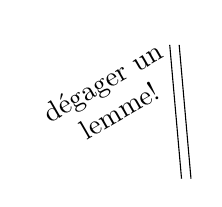
\begin{tikzpicture}[x=1cm,y=1cm]
\node[rotate=30,align=center] at (0,.9) {\unsure{dégager un}\\\unsure{lemme}!};
\draw (.9,-.15)--(.75,1.55) (1.02,-.15)--(.87,1.55);
\end{tikzpicture}}}
